%% 
\chapter{Optimizing Species-Specified Aerosol Emissions} \label{chap:optems}

\section{Introduction}

 In this chapter, we present a new attempt for the top-down estimate 
 of aerosol emissions through integration of the satellite observation 
 of reflectance and GEOS-Chem Adjoint model. 
 The technique is applied to improve estimates of mineral dust 
 and anthropogenic \ce{SO2}, \ce{NH3}, \ce{NOx}, \ce{BC} and \ce{OC} 
 emissions over China for April 2008, during which ground-based 
 PM\textsubscript{10} (particulate matter with aerodynamic diameter of 
 10 $\mu$m or less) data is available from a joint China-U.S. 
 dust field experiment [Huang et al., 2010]. 
 This paper differs from the past work in that: 
 (i) satellite reflectance (in essence radiance) is used 
 to constrain the emission estimates of aerosol particle and precursors, 
 which eliminates the discrepancy of aerosol optical properties 
 between model simulated and satellite retrieved AOD; 
 (ii) we use a suite of aerosol and gas measurements 
 from satellite sensors and ground-based instruments 
 to independently evaluate our results, and test our hypothesis 
 that temporal variation of AOD at different locations, 
 as characterized by satellite observations, can be a strong constraint 
 for species-specific source estimates if they are combined with 
 the model-based knowledge of the dominant aerosol sources 
 and the source-receptor relationship at corresponding locations; 
 and (iii) combination of (i) and (ii) will provide the basis and 
 a necessary step forward for future research to simultaneously 
 use both gas and AOD measurements to constrain speciated aerosol emissions. 

 We describe the top-down inversion scheme and its key components 
 (i.e., GEOS-Chem forward model and its adjoint, and observational constraints) 
 in Section 2. The top-down constraints on aerosol emissions over China 
 for the period of April 2008 are presented in Section 3, 
 and evaluated in Section 4. Interpretation and 
 implications of the results are discussed in Section 5, 
 and Section 6 summaries this study. [needs updates!!!!]

 \begin{figure}[ht]
  \centering
  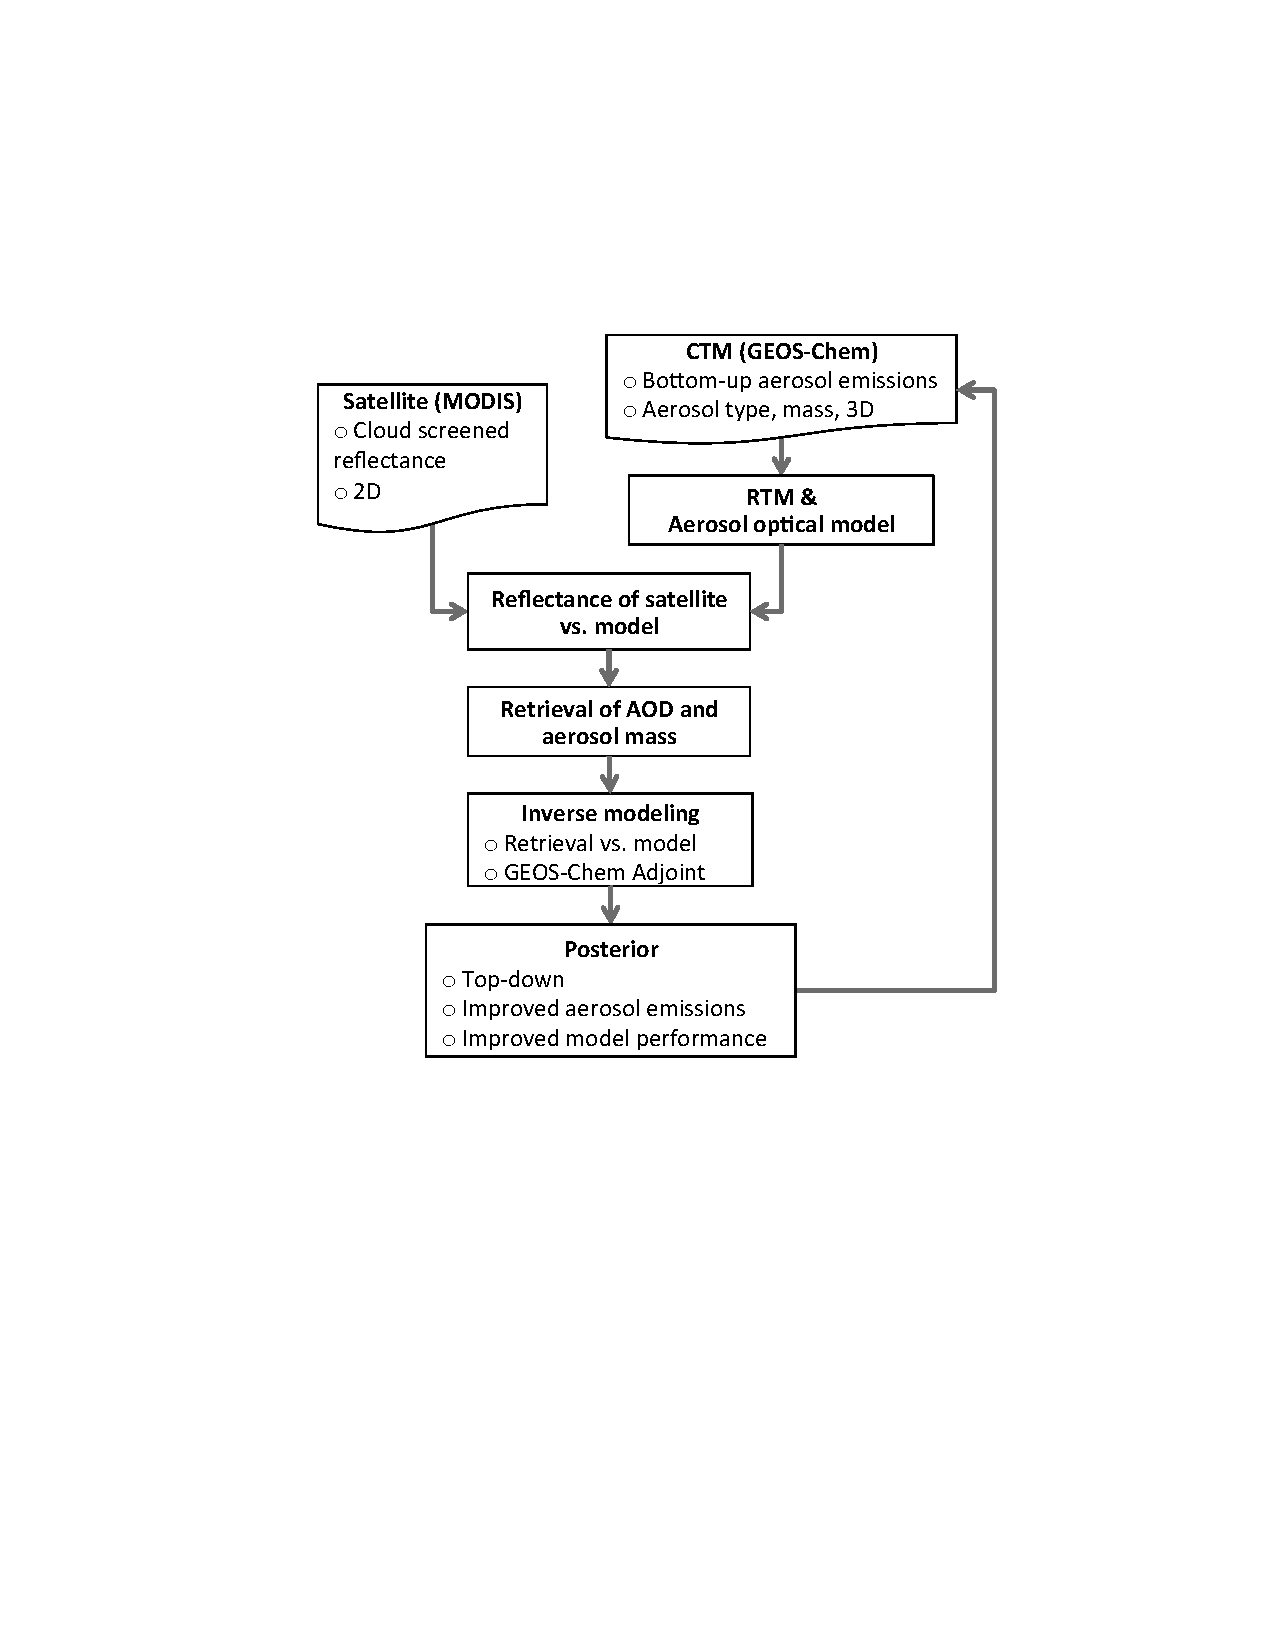
\includegraphics[width={0.7\textwidth}]{figures/a1.pdf}
  \caption{Flowchart of the proposed top-down inversion framework.}
  \label{fig:flowchat}
 \end{figure}

 As shown in Figure \ref{fig:flowchat}, the top-down inversion approach in this study 
 integrates the MODIS radiance/reflectance with the GEOS-Chem (section 2.1) 
 and its adjoint model (section 2.2) to optimize aerosol emissions. 
 First, similar to Wang et al. [2010], we retrieve the atmospheric 
 aerosol mass and AOD through fitting the calculated radiance based on 
 GEOS-Chem aerosol composition and single optical properties to the MODIS 
 cloud-free radiances (section 2.3). Second, the retrieved AOD 
 (hereafter retrieved MODIS AOD) from the first step is used as 
 an observational constraint to optimize the aerosol emissions 
 by inverting the GEOS-Chem chemical transport model (section 2.4). 
 The approach aims to improve aerosol emission estimates that ultimately 
 will yield better agreement between model simulated and satellite-observed 
 reflectances.  Since the aerosol single scattering properties are 
 exactly the same between the retrieval algorithm and GEOS-Chem 
 (as done in the first step), the top-down inversion scheme essentially 
 uses the MODIS radiances (in the form of retrieved AOD) to scale the 
 GEOS-Chem aerosol mass, which in turn are used to optimally adjust 
 the aerosol emissions. The approach here is first demonstrated through 
 a pseudo-observation experiment (Section 2.5) before it is applied 
 to real observations (Section 3).

\section{Constraints from Satellite Radiances}

 The observational constraints in this study are 
 MODIS reflectances from both Terra and Aqua satellites, 
 from which four-dimensiaonal mass concentrations of six aerosol species 
 (namely, \ce{SO4}, \ce{NO3}, \ce{NH4}, BC, OC, and dust) have been derived 
 with the GEOS-Chem model using the retrieval algorithm presented by Wang et al. [2010]. 
 Key to this algorithm are: 
 (a) a database of time-dependent local 0.65 and 2.1 $\mu$m surface reflectance ratio 
 that are derived from samples of the MODIS dark-pixel reflectance data in low AOD conditions 
 (i.e. dynamic lower envelope method), 
 (b) an assumption that the simulated CTM aerosol is unbiased 
 in composition and vertical distribution shape but possibly largely biased 
 in total mass or optical depth, 
 and (c) a linearized radiative transfer model (VLIDORT [Spurr, 2006]) 
 that computes the top-of-atmosphere (TOA) reflectance 
 and its Jacobian sensitivity to the column AOD using 
 the GEOS-Chem single aerosol optical properties 
 and the solar-earth-sensor geometries of the coincident MODIS scene. 
 With above (a), (b), and (c), Wang et al. [2010] retrieved two unknowns 
 (AOD at 0.65 $\mu$m and surface reflectance at 2.13 $\mu$m) 
 from two MODIS observed quantities (0.65 and 2.13 $\mu$m TOA reflectance) 
 by seeking the minimum differences between GEOS-Chem and MODIS reflectance. 
 Based on (b), mass concentrations of individual aerosol species 
 at each MODIS overpassed grid cell are updated by applying the AOD scaling factors 
 (ratios of retrieved AOD to GEOS-Chem AOD at 0.65 $\mu$m) 
 and are used as observational constraints for optimizing aerosol emissions. 
 According to the evaluation of the retrieved AOD against AERONET AOD [Wang et al., 2010], 
 we found the uncertainty is generally less than 20\%, 
 which we subsequently use to quantify the observation error 
 in the inverse modeling optimization. 

 GEOS-Chem simulated aerosol composition over Asia is shown by multiple studies 
 to have large underestimation in BC, and equivalent or larger underestimation 
 of OC mass and overestimation of sulfate aerosol mass [Heald et al., 2005; Fu et al., 2012], 
 which suggests that the mass fraction of highly absorbing (BC) 
 and highly scattering (OC and sulfate) fine mode aerosols may have far less biases 
 (as compared to the relative bias in OC mass only). 
 Consequently, no significant biases are assumed for: 
 (a) the GEOS-Chem simulated fraction of coarse mode (dust) aerosol mass, 
 and (b) the GEOS-Chem simulated aerosol single scattering albedo. 
 While (b) is important to ensure an unbiased retrieval of AOD, 
 (a) supports that the GEOS-Chem simulated dust AOD fraction is likely unbiased, 
 both of which support the use of AOD scale factors derived from MODIS 
 for constraining emission of coarse-mode dust and fine-mode aerosols. 
 Admittedly, any model bias in modeled AOT fraction for each individual species 
 can lead to a corresponding bias (of the same sign) in the adjoint modeling 
 results for individual emission. 
 Quantification of such bias is not possible for the present study 
 owing to the lack of aerosol composition data in China.

\section{Inversion Strategies}

\subsection{Selection of emissions for optimization} \label{sec:selectems}

 The inversion scheme and the MODIS-based constraints, as described in the last three sections, 
 are combined to constrain the aerosol emissions over the Eastern Asia 
 for the period of April 2008. 
 The modeled emission parameters that most significantly influence the discrepancy 
 between simulation and observations are selected and spatially constrained. 
 Specifically, those model parameters (or control parameters) represent six emitted tracers, 
 as listed in Table 2, which include emissions of \ce{SO2}, \ce{NH3}, and \ce{NOx}, BC, 
 and OC from anthropogenic sources, and mineral dust. 
 Bottom-up inventories (and an online mobilization scheme for dust) are used as 
 \textit{a priori} estimates, corresponding magnitudes and geographic distributions 
 of which are shown in Table 2 and Figure \ref{fig:ems1}, respectively. 
 The temporal extent of the optimization window is selected 
 to be reconcilable with the temporal variability of the bottom-up emission. 
 We set optimization window of a month for those trace gases and carbonaceous emission tracers; 
 while dust emission tracers are constrained daily in a separate optimization run 
 following approach by Wang et al., [2012]. 
 Both optimizations assimilate hourly observations during the adjoint simulation. 

 The 4D-Var technique in the optimization requires background 
 error covariance statistics for each control parameter. 
 We specify the priori error for those emission tracers 
 based on characterized spatial and temporal averaged uncertainties for those inventories 
 [Zhang et al., 2009; Bond et al., 2007; Zender et al., 2003] 
 but with larger values to reflect the possibly large local aerosol emission 
 uncertainties in the bottom-up inventories. 
 The uncertainty for \ce{SO2} emission estimate is believed 
 to be smaller than those for \ce{NH3} and \ce{NOx}, 
 while uncertainties of other tracers could be even larger 
 [Textor et al., 2006; Zhang et al., 2009]. 
 Therefore, we set relative error of 50\% for \ce{SO2}, 100\% for \ce{NH3} and NOx, 
 200\% for BC, OC, and dust sources. 
 Lacking information to fully construct a physically representative 
 prior error covariance matrix, a regularization parameter $\gamma$ 
 is introduced in the cost function to balance the contribution of model error and source error,  with a value (here $\gamma = 1000$) selected using the L-curve technique [Hansen, 1998]. 
 Moreover, in order to test the impact of those specified uncertainties on the optimization, 
 we run a case with an arbitrary prior error of 100\% for all emission tracers, 
 and present the results in Table 3. 

 \subsection{Sensitivity test with pseudo AOD observations}

 We first conduct a pseudo experiment to assess: 
 (1) the concept that temporal variations and geophysical location of AOD, 
 when interpreted with GEOS-Chem model, 
 can yield information about change regarding aerosol composition and emissions, 
 and (2) the sensitivity of the inversion results to the assumption 
 that GEOS-Chem simulated relative composition or single scattering albedo of aerosol is unbiased.
 The experiment has three steps:
 (a) GEOS-Chem simulation with standard bottom-up EIs 
 are first conducted to obtain prior aerosol composition 
 and 0.65 $\mu$m AOD for the period from April 5 to 11 of 2008; 
 (b) Pseudo-observations of AOD are created by perturbing the following emissions 
 (relative to bottom-up EIs) in GEOS-Chem: +20\% for \ce{SO2}, \ce{NH3}, and \ce{NOx}, 
 -40\% for dust, and zero for BC and OC (Table 1); 
 (c) These pseudo-observations of AOD in the dark surface region (red box in Figure 2a), 
 twice per day, respectively at the Terra and Aqua overpass daytime, 
 are subsequently used as truth to constrain emissions using the GEOS-Chem adjoint-based inversion. 

 \begin{figure}[t]  \centering  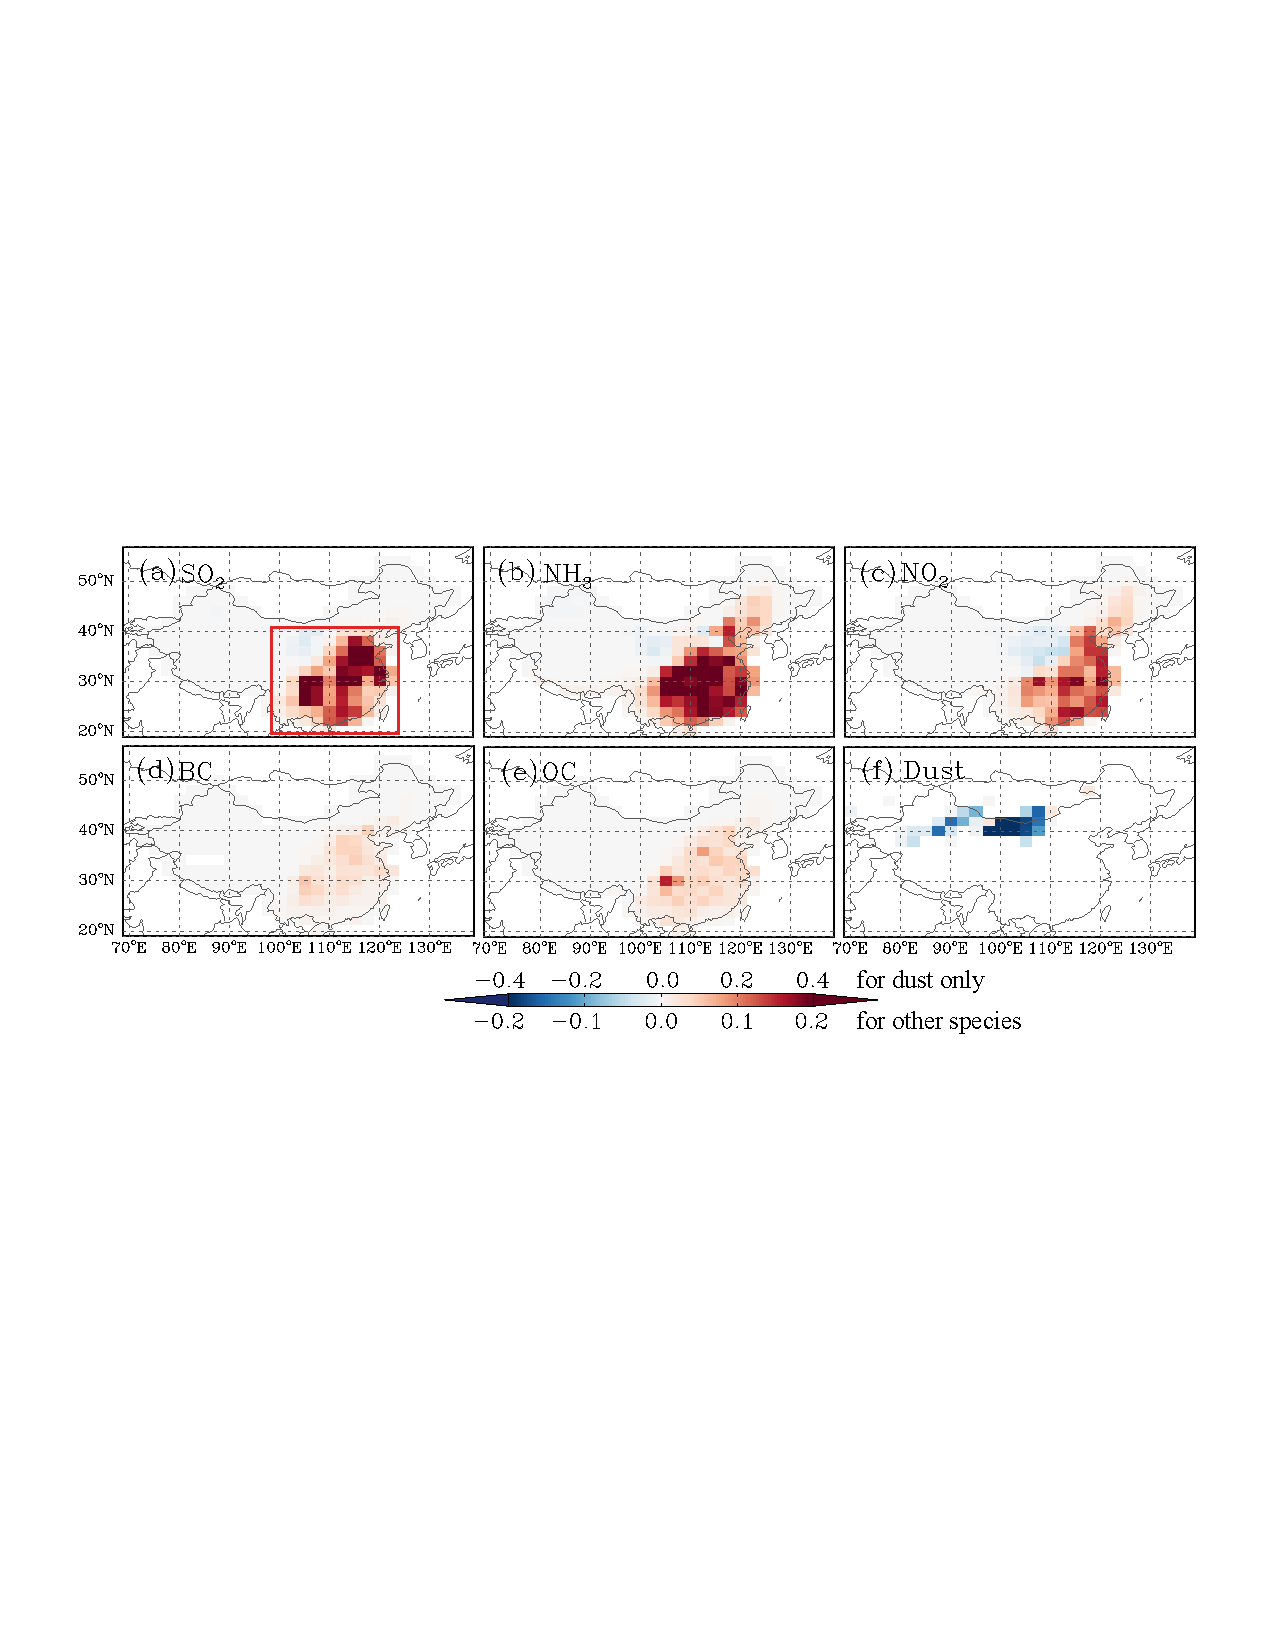
\includegraphics[width={0.95\textwidth}]{figures/a2.pdf}
  \caption{Relative changes in posterior aerosol emissions from \textit{a priori}
   in the pseudo-observation experiment.
   Six panels are respectively for anthropogenic emissions of \ce{SO2}, \ce{NH3},
   \ce{NOx}, BC, and OC, and mineral dust from both natural and anthropogenic sources.
   The red box in panel (a) indicates the region where AOD observations are selected. }
  \label{fig:pseudo1}
 \end{figure}

 The degree to which the inversion can correct for species-specific errors in the emissions 
 is assessed in these sensitivity tests by comparing the optimized aerosol emissions 
 from (c) can then be evaluated against the truth, or the perturbed emissions in (b).  
 Figure \ref{tab:pseudo1} shows the distribution of relative changes in posterior emissions 
 from the 6th iteration with respect to the prior bottom-up emissions for each species; 
 the overall changes over the China are shown in Table \ref{tab:pseudo1}.
 By the 6\textsuperscript{th} iteration, the cost function reduced by 50\%; 
 further iterations yielded negligible additional decreases. 
 The posterior emissions for \ce{SO2} and \ce{NH3}, which increased by 14\% from the prior, 
 are close to the “truth” (20\%). \ce{NOx} emissions were increased by 8\%, 
 a smaller change than \ce{SO2} and \ce{NH3}. 
 Dust emissions reduced by 26\% percent in the inversion, 
 approaching the true values of -40\%.
 BC and OC emissions were increased by 2\% and 3\%, which are close to the truth of 0. 

 Overall, this sensitivity study demonstrates that the inversion is capable of resolving the sign,
 spatial distribution, and the bulk of the true perturbations for the emissions of each species.
 Meanwhile, we also note that the adjoint inversion could transfer (somewhat marginal) errors
 from one tracer to another, such as increases in BC and OC emission 
 as a result of significant underestimations in the prior \ce{SO2}, \ce{NH3}, and \ce{NOx} emissions,
 reflecting errors due to assumptions related to unbiased GEOS-Chem aerosol composition.
 We can also assume that similar aliasing would occur in attempts 
 to distinguish the impacts of co-located precursor emissions of scattering particles
 (e.g., \ce{SO2} and \ce{NOx} from power plants),
 although additional tests would be necessary to assess whether or not differences 
 in the timescales (and thus transported length scales) 
 over which these emissions impact AOD would allow their sources to be separated.
 Long-range transport of dust appears to have less influence on the inversion because:
 (a) except dust, there are little (other) emissions in dust source regions;
 (b) a sudden increase of AOD in downwind regions can be interpreted by GEOS-Chem
 due to the dust transport, and this increase can be used by GEOS-Chem adjoint
  as constraint to optimize the dust emission.

\begin{table}[t]
  \centering
  \small
  \caption{Prior, posterior, and perturbed aerosol emissions over China in the pseudo experiment.}
  \label{tab:pseudo1}
  \begin{tabular}{>{\centering\arraybackslash}m{0.10\textwidth}
                  >{\centering\arraybackslash}m{0.15\textwidth}
                  >{\centering\arraybackslash}m{0.15\textwidth}
                  >{\centering\arraybackslash}m{0.15\textwidth}
                  >{\centering\arraybackslash}m{0.15\textwidth} }\toprule
    Tracer & $E_\text{prior}$ (Gg/Month) & $E_\text{posterior}$ (Gg/Month)& $E_\text{posterior}/E_\text{prior}$ (\%)& $E_\text{perturbed}/E_\text{prior}$ (\%)\\ \midrule
    \ce{SO2} & 520.8 & 592.0 & 113.7 & 120 \\
    \ce{NH3} & 219.3 & 249.2 & 113.7 & 120 \\
    \ce{NOx} & 338.8 & 365.3 & 107.8 & 120 \\
    BC & 23.3 & 23.8 & 102.3 & 100 \\
    OC & 39.7 & 41.1 & 103.4 & 100 \\
    Dust & 2301 & 1697 & 73.7 & 60 \\ \bottomrule
  \end{tabular}
\end{table}

\section{Inversion Results}

 \begin{figure}[ht]
  \centering
  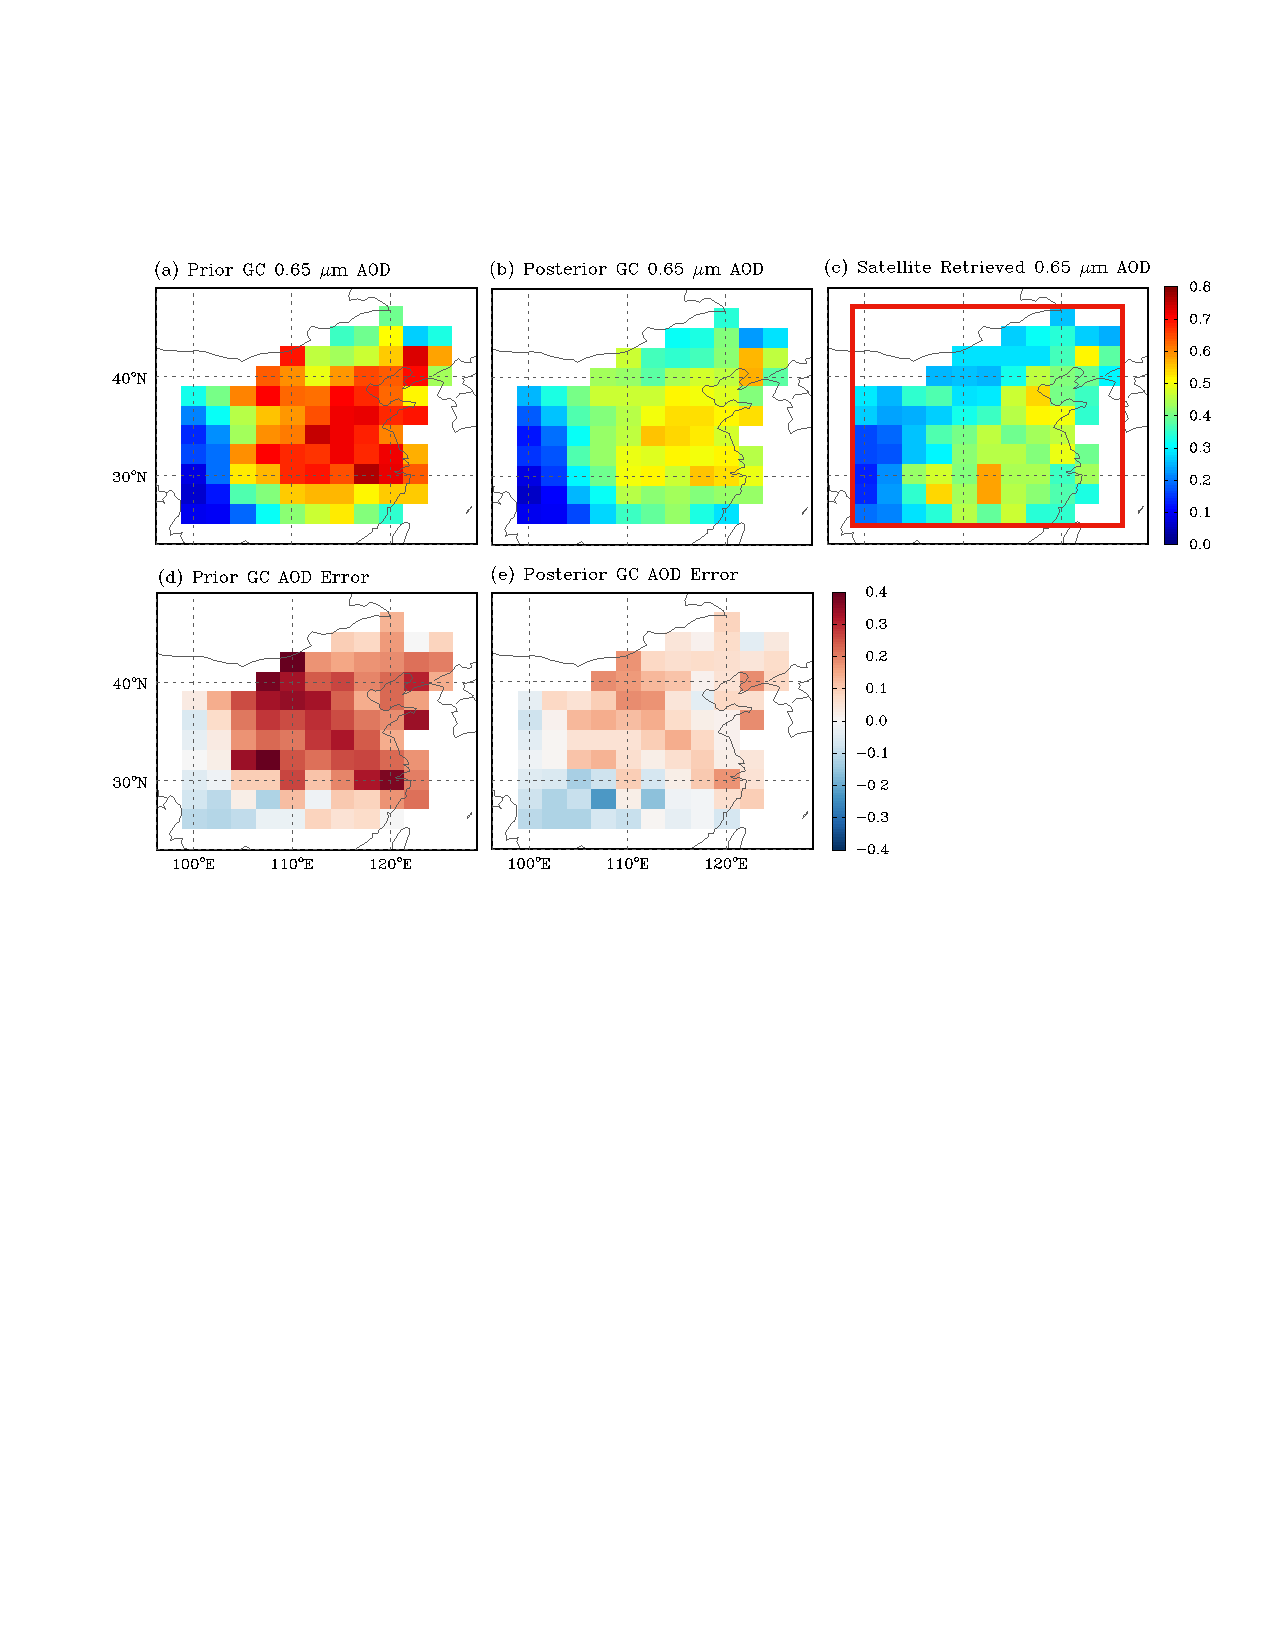
\includegraphics[width={0.95\textwidth}]{figures/a3.pdf}
  \caption{Comparison of the prior (a) and posterior (b) GEOS-Chem (GC) simulation
 of 0.65 $\mu$m AOD with the AOD at the same wavelength retrieved from
 MODIS reflectance using GEOS-Chem aerosol optical properties (c) averaged
 for the period of April 2008. Satellite retrievals with 10 km by 10 km at nadir
 are aggregated to GEOS-Chem grid cells; and the model AOD are sampled coincidentally
 with those retrievals. Panel (d) and (e) respectively show the difference of
 prior and posterior simulated from the satellite retrieved AODs.
 The red box in panel (c) indicates the region where AOD observations are selected.}
  \label{fig:aod1}
 \end{figure}

 With the feasibility of the approach demonstrated in Section 2, 
 we apply the approach to MODIS radiance data in April 2008. 
 The emissions that result from each iteration during the optimization 
 enable GEOS-Chem to produce a different set of AOD values 
 that converge to the observational constraints. 
 Figure \ref{fig:aod1}c shows the geographic distribution of GEOS-Chem AOD at 0.65 $\mu$m, 
 simulated with prior aerosol emissions, averaged coincidently with retrieved daily MODIS AOD 
 (Figure \ref{fig:aod1}c) during April 2008. 
 While the prior model simulation captures the overall spatial pattern of AOD 
 with larger values over eastern China, 
 it has a slight underestimation over the southwestern China 
 but an overwhelming overestimation elsewhere, 
 when compared to the retrieved AOD from MODIS radiance (Figure \ref{fig:aod1}d). 
 The optimization is expected to adjust aerosol emissions to reduce those differences. 
 Following the experiment design described in section \ref{sec:selectems}, 
 we find that after 6 iterations of the GEOS-Chem forward and adjoint runs, 
 the cost function is reduced by about 60\%, 
 and further iterations yield negligible reductions in the cost function. 
 Therefore, the aerosol emissions adjusted in iteration 6 are selected as the final optimal results. 
 As shown in Figure \ref{fig:aod1}b and \ref{fig:aod1}e, the posterior GEOS-Chem AOD 
 that are simulated with the optimized aerosol emissions 
 are in much better agreement with their counterparts retrieved from MODIS reflectance, 
 which is also reflected by the cost function reduction and 
 confirms the effectiveness of the adjustment in top-down emissions.

 %% Figures of the daily variations in the AOD and dust emission
 \begin{figure}[p]
  \centering
  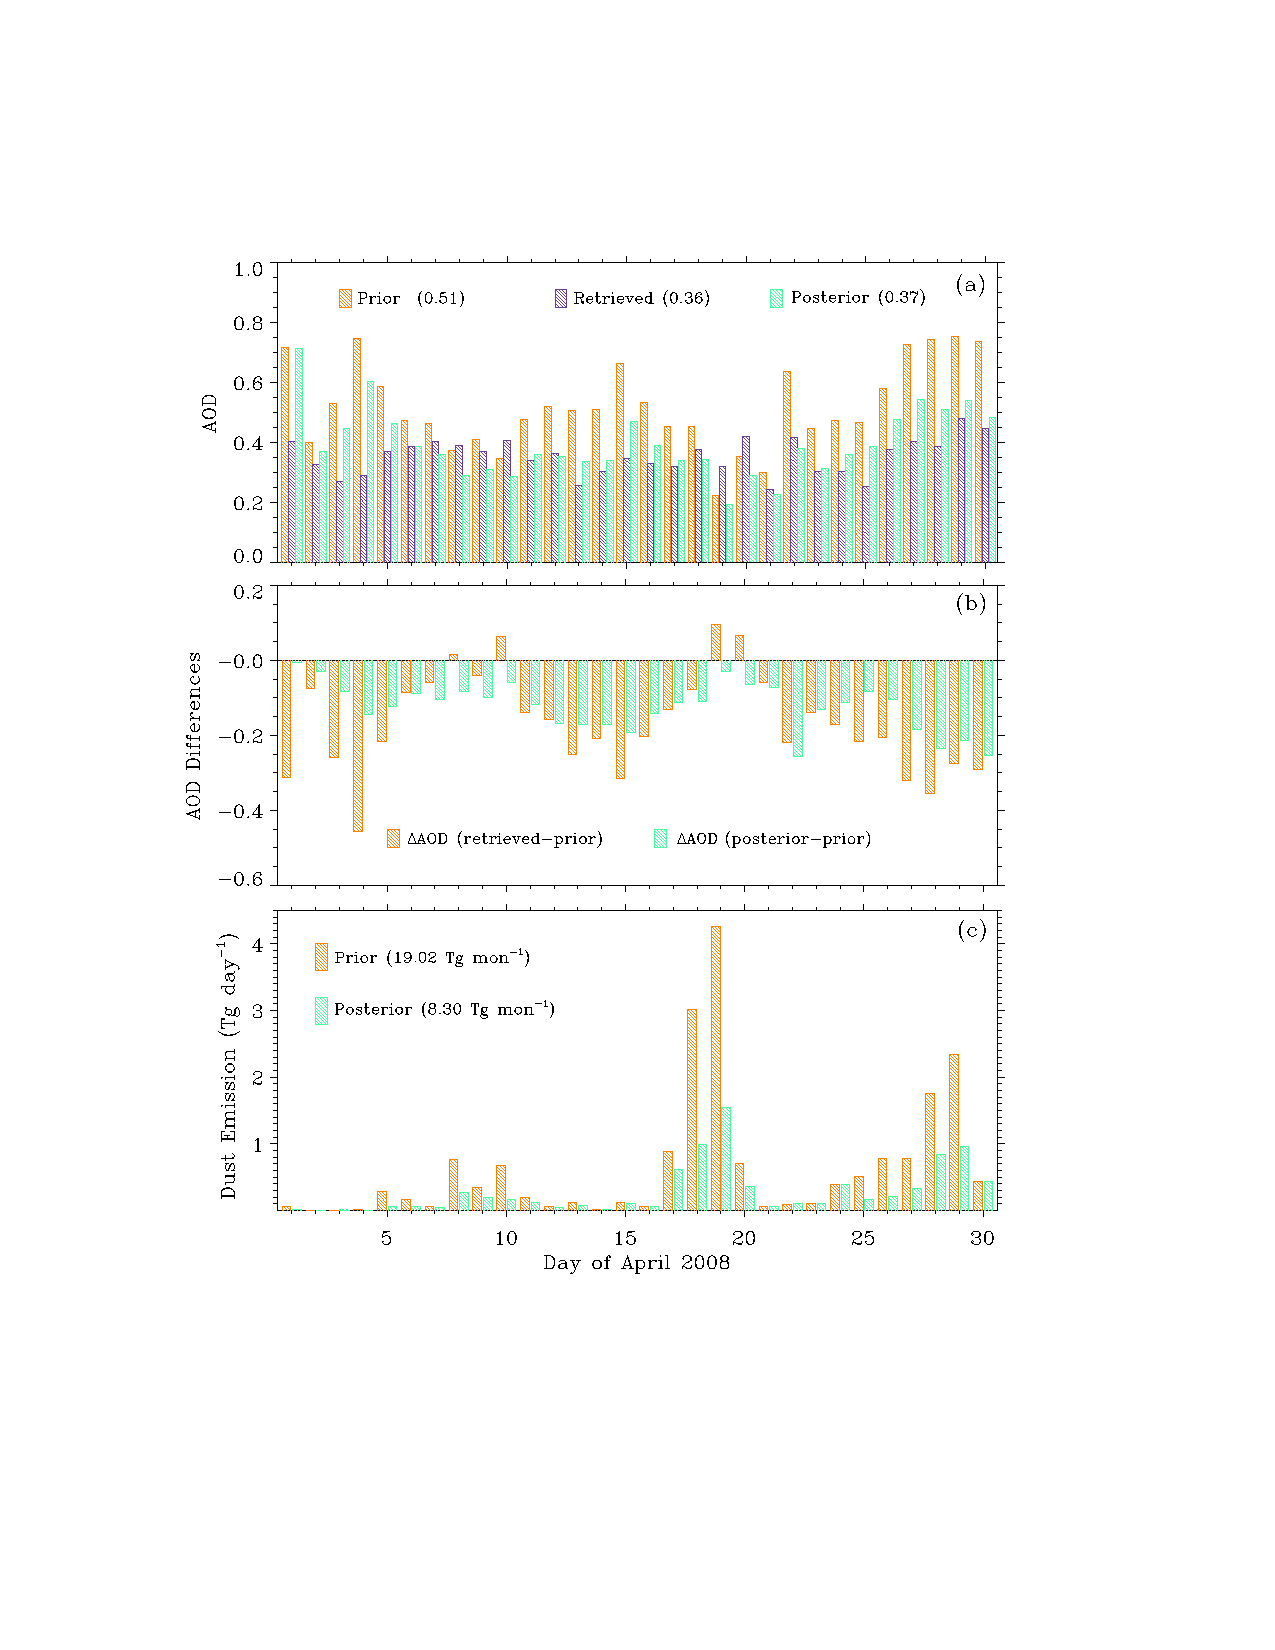
\includegraphics[width={0.8\textwidth}]{figures/a4.pdf}
  \caption{(a) Time series of the spatially averaged daily MODIS AOD retrievals (purple) for April 2008 over the Eastern China, compared by the prior (orange) and posterior (green) spatial averaged daily GEOS-Chem AOD that are sampled in the MODIS AOD tempo-spatial space. (b) Time series of the expected daily AOD adjustments (orange) that are the differences between MODIS AOD and the prior GEOS-Chem AOD and their real adjustments (green) that are the differences of posterior from prior GEOS-Chem AOD. (c) Time series of the prior (orange) and posterior (green) daily dust emissions over China for April 2008.}
  \label{fig:dailyaod}
 \end{figure}

 The convergence of the model simulation to the MODIS AOD retrievals 
 is also indicated in the AOD daily variability. 
 Figure \ref{fig:dailyaod}a shows the daily variations of the AOD 
 spatially averaged for available MODIS retrievals (purple) over the eastern China areas 
 within the red box in Figure \ref{fig:aod1}c, and the coincidental GEOS-Chem simulation
 prior and posterior to the aerosol emission optimization (orange and green, receptively).
 The prior model produce overestimated AODs for most days during the month.
 After top-down adjustments to the aerosol emissions,
 such overestimation of the AOD is reduced in total over the course of the month.
 As shown in Figure \ref{fig:dailyaod}b, the real changes of the modeled daily AOD 
 during the optimization (green bars), or equivalently, the differences of the posterior
 from the prior are consistent with the expected changes, i.e.,
 the differences of the MODIS retrievals from the prior model simulation.
 It is noted that the posterior AODs has larger departure from the observation
 than the prior on a few days.
 This reflects that monthly-scaled emissions are not perfectly capturing the daily variation of emission.

 %% Figures of the optimized ems
 \begin{figure}[p]
  \centering
  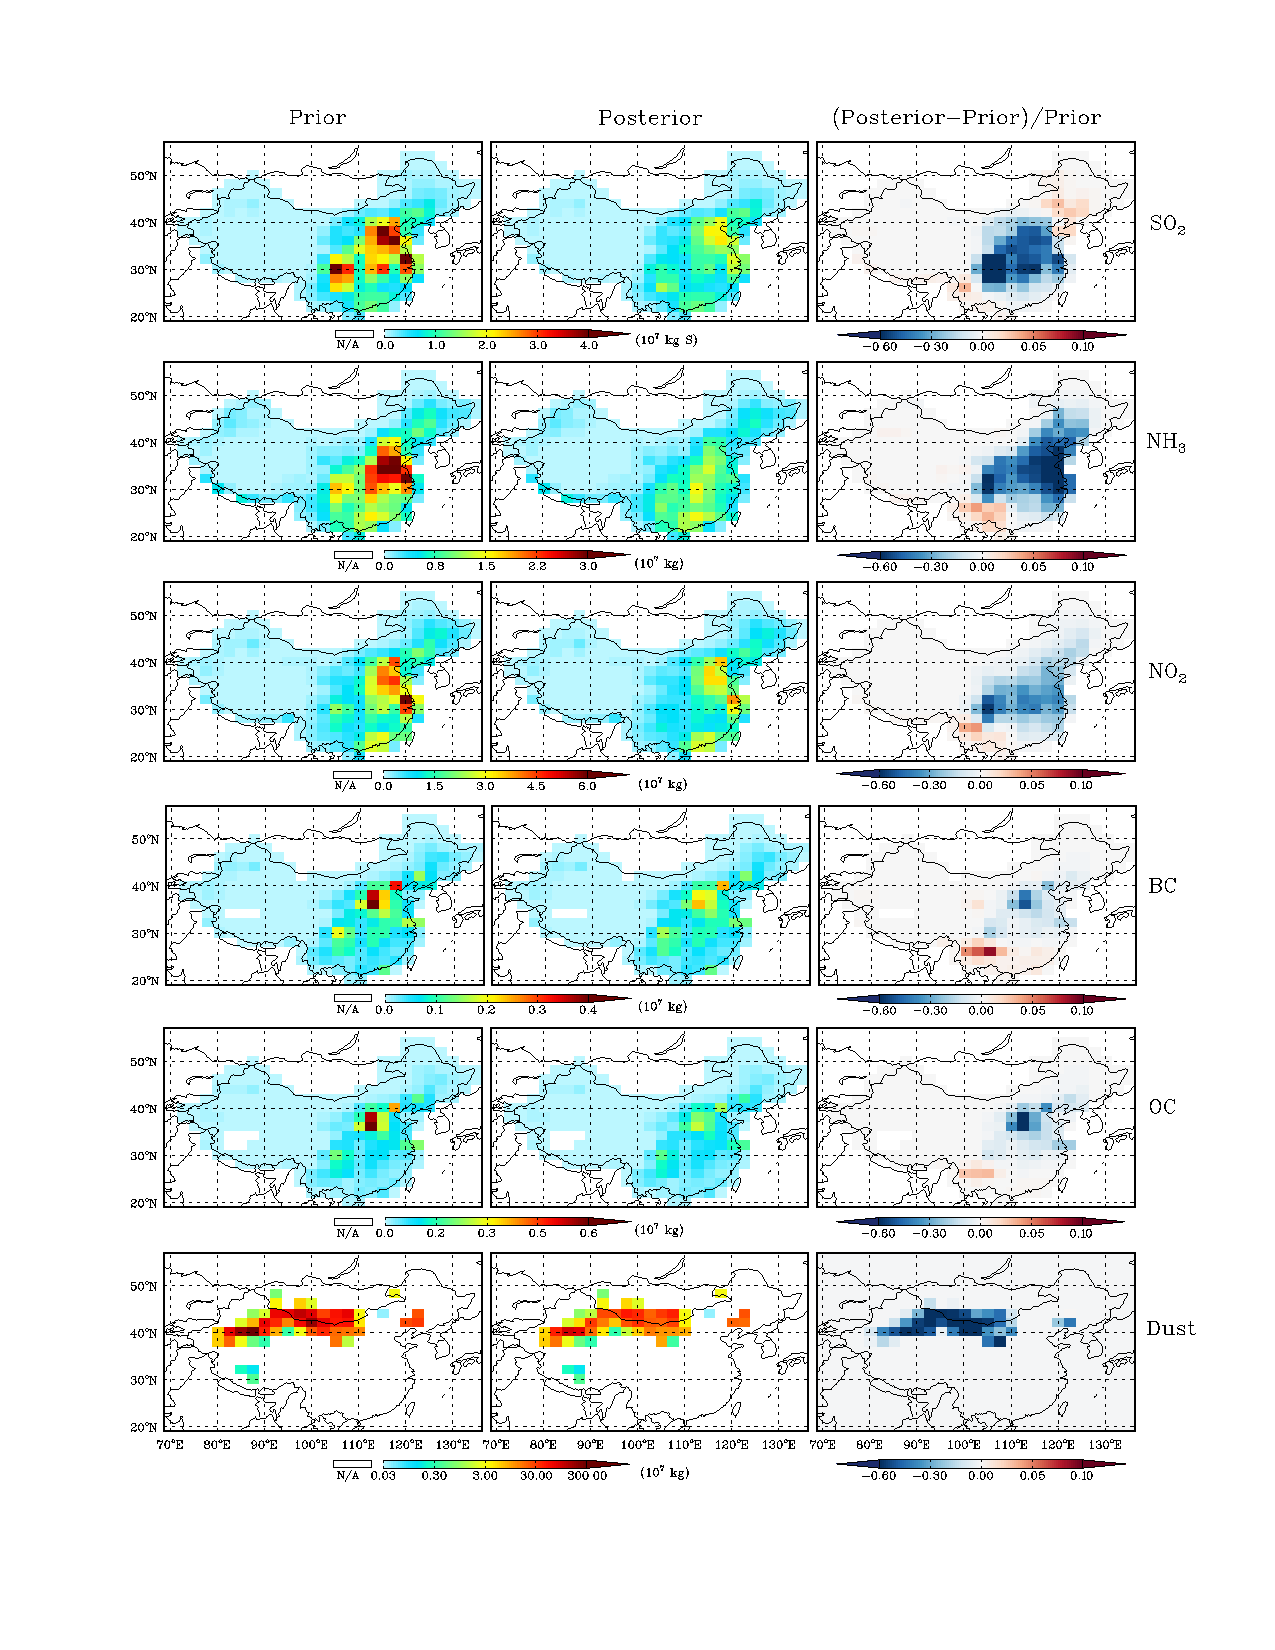
\includegraphics[width={0.95\textwidth}]{figures/a5.pdf}
  \caption{The prior (or bottom-up based, left column), optimized (or top-down constrained, middle column) aerosol emissions over China for the period of April 2008, and their relative differences (right column). Six rows from top to bottom are respectively for anthropogenic emissions of \ce{SO2}, \ce{NH3}, ce{NOx}, BC, and OC, and mineral dust from both natural and anthropogenic sources. }
  \label{fig:ems1}
 \end{figure}

 Emissions of \ce{SO2}, \ce{NH3}, \ce{NOx}, BC, and OC from anthropogenic sources
 are optimized monthly and rescaled over each individual
 2$^{\circ}$ by 2.5$^{\circ}$ grid cell of China for the month of April 2008.
 The prior and posterior (optimized) emissions of those tracers
 are respectively shown in left and middle columns of Figure \ref{fig:ems1},
 in which the relative changes of those emissions in the optimization
 are also included in the right column. Overall, the optimization yields
 an overwhelming reduction for all emission tracers,
 even though some local increases are found.
 As expected, such adjustment in the constrained aerosol emissions
 is consistent with the changes in GEOS-Chem AOD before and after optimization,
 as aerosol loadings usually positively respond to the aerosol emissions.
 Quantitatively, anthropogenic emissions over China continent for the study period
 are changed by $-$33.5\% for \ce{SO2} from 1.302 to 0.866 Tg, -34.5\% for \ce{NH3} from 1.096 to 0.718 Tg,
 -18.8\% for \ce{NOx} from 1.694 to 1.375 Tg, -9.1\% for BC from 0.11 to 0.10 Tg,
 and -15.0\% for OC from 0.205 to 0.175 Tg (Table 2).
 The largest reduction occurs sharply in the central regions of the Eastern China,
 corresponding to the region where the largest AOD are adjusted to the MODIS retrievals.
 Small increases of emitted anthropogenic sources of gases and carbonaceous particles
 are found over the southwestern China, which can be explained
 as the response for the underestimation of AOD in the model simulation over these regions
 (Figure \ref{fig:aod1}a, d). 

 The mineral dust emissions from both anthropogenic and natural sources are optimized daily.
 The adjoint has no leverage to increase the dust emissions over grid cells
 having zero dust emission in the priori estimate identified by the modified DEAD scheme.
 Thus, the posteriori dust source region remains un-shifted as shown
 in Figure \ref{fig:ems1} (bottom panels), which is reasonable
 because the expansion or shrinkage of desert regions is unlikely to extend beyond
 the grid size (2$^{\circ}$ by 2.5$^{\circ}$) of this study \citep{zender03a,fairlie07}.
 The total amount of the optimized dust emissions for April 2008 over China is 8.3 Tg,
 reduced by 56.4\% from the modified DEAD module simulation of 19.02 Tg.
 Such reduction indicates an overestimation in the prior emissions of dust,
 especially over Gobi deserts that are located in the Northwestern China and the southern Mongolia.
 Wang et al. [2012] presented a similar result,
 but only for a dust event that occurred in the later portion of our study time period.
 Figure \ref{fig:dailyaod}c illustrates the time series of the prior and optimized
 daily total dust emission.
 Two sharp peaks of the dust emissions indicate the occurrences of strong dust storms
 after April 15. Such large temporal variation in the daily scale
 requires the optimization of dust emission on the daily basis. 

 An additional case with specified error of 100\% for all the anthropogenic emission tracers
 is conducted to examine the sensitivity of those specified error to the optimization.
 Table 3 shows the relative change in optimized emissions for two different scenarios.
 Less than 0.5\% difference in the optimized emissions is found,
 which means the uncertainty in a priori emission could have
 much smaller impact on the optimization than the observational constraints.

\section{Results Evaluations} 

 Because direct measurements of the aerosol emissions are few over China,
 we assess the optimized sources by comparing the GEOS-Chem posterior
 simulated aerosol mass concentrations and AOD with
 the independent observations from various sources.
 The evaluation datasets include:
 (1) AERONET AOD observations [Holben et al., 1998] over nine sites;
 (2) Level 3 MISR daily AOD products [Kahn et al., 2005];
 (3) Level 3 SO2 [Krotkov et al., 2006; Lee at al., 2009]
 and Level 2 NO2 [Bucsela et al, 2006] retrievals from the Ozone Monitoring Instrument (OMI);
 (4) surface mass concentration of sulfate-nitrate-ammonium (SNA) aerosol particles over Qingdao, China;
 and (5) surface PM10 over two sites close to dust source region [Ge et al., 2010]. 

 \subsection{Comparison with AERONET AOD}

 We first evaluate the prior and posteriori GEOS-Chem 0.55 $\mu$m AOD against
 the AERONET AOD at 0.55 $\mu$m that are interpolated from AODs at 0.44 and 0.67 $\mu$m
 based on the Angstrom exponent.
 Three-hour averaged values of available AERONET AOD,
 centered by the model output time are used to compare with
 the model AOD over the grid cells locating the AERONET sites.
 The scatterplots shown in Figure \ref{fig:aeronet} are the comparisons
 for nine stations over China, South Korea, and Japan representing different aerosol types.
 The first three stations, i.e., (a) Zhangye, (b) SACOL, and (c) Jingtai,
 which are located over rural regions in the south boundary of Gobi deserts
 and have little influence from anthropogenic emissions,
 are representative sites for dust aerosol [Ge et al., 2010].
 The next three sites, (d) Beijing, (e) Xinglong, and (f) Heifei,
 are located in anthropogenic source regions.
 The last three sites, (g) Noto, (h) Shirahama, and (i) Gwangju\_K,
 are located over Japan and South Korea, the downwind regions of China emissions.
 Those last six stations are affected not only by the local anthropogenic emissions
 but also by the long-range transported aerosols from the upwind regions.
 Indeed, those three categories of stations are respectively located
 in the upwind, central, and downwind of regions having the observational constraints.

 %% Validation vs AEORNET
 \begin{figure}[t]
  \centering
  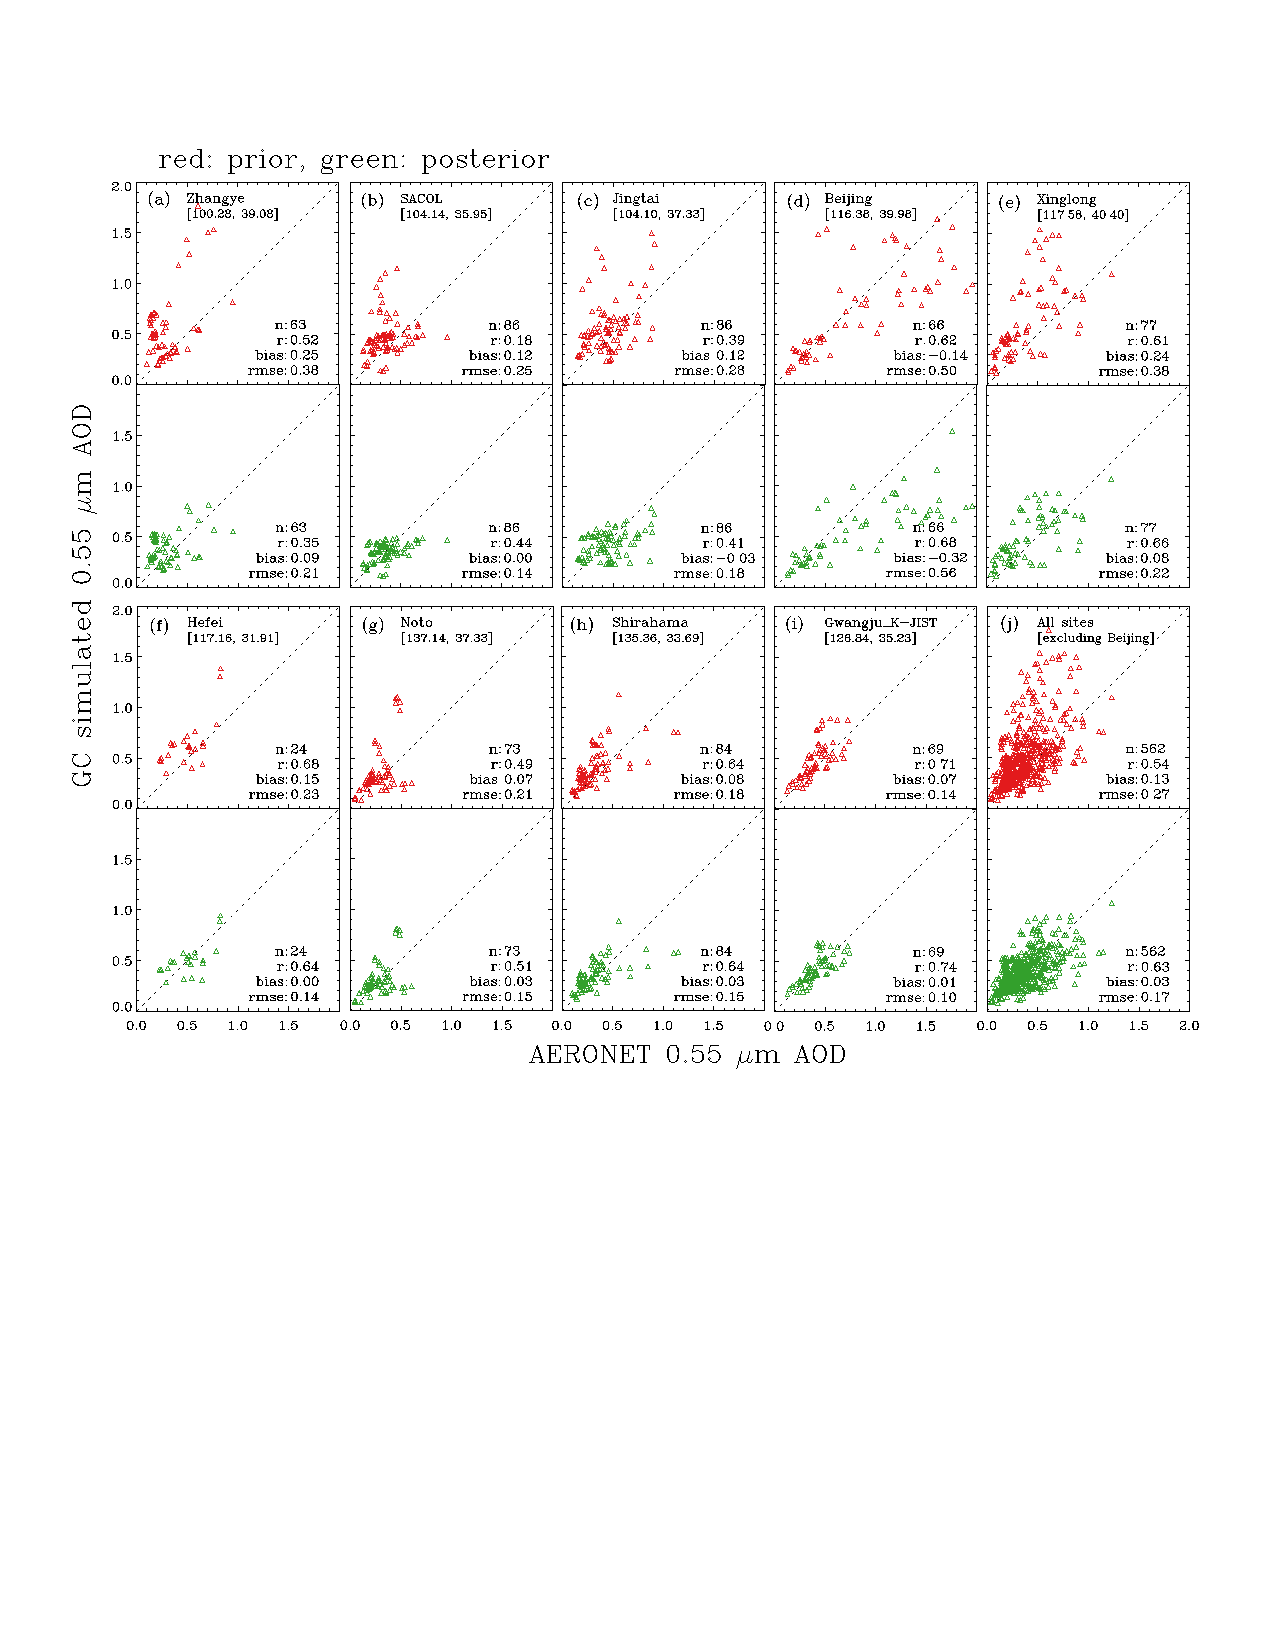
\includegraphics[width={0.99\textwidth}]{figures/a6.pdf}  
  \caption{(a – i) Scatterplots of GEOS-Chem AOD versus AERONET AOD at 0.55 $\mu$m prior (red scatters) and posterior (green scatters) to the aerosol emission optimization over nine stations. AERONET AODs are 3-hour averages following the GEOS-Chem output frequency. (j) The overall comparison for eight AERONET sites excluding Beijing. Also shown are the number of valid sampled pairs (n), correlation coefficients (R), bias, and root-mean-square-error (rmse).}
  \label{fig:aeronet}
 \end{figure}

 The prior GEOS-Chem simulation (shown in the red scatter panels)
 overestimates the AERONET AOD for all the sites except Beijing.
 The low bias of model AOD at Beijing is likely owing to the model coarse resolution,
 which fails to resolve heavy local urban pollution.
 The geographic area of urban Beijing is about 1300 km\textsuperscript{2}
 (\url{http://en.wikipedia.org/wiki/Beijing}),
 less than 3\% of the area of a GEOS-Chem grid cell.
 Thus, the local pollution signal is smeared in the model grid box.
 Moreover, Beijing and Xinglong are in the same model grid cell,
 but AERONET AOD over Xinglong is much smaller than that over Beijing site
 (as later shown as circles on the maps of Figure \ref{fig:misr1}a-c).
 As Beijing site is difficult to represent in the GEOS-Chem at 2$^{\circ}$ by 2.5$^{\circ}$ resolution,
 we exclude Beijing site in our further analysis.
 GEOS-Chem AOD from the posterior aerosol emissions are in more agreement with the AERONET AOD
 (shown in the green scatter panels),
 as indicated by reduced bias and root-mean-square-error (rmse) over all the other sites and
 increased correlation coefficients (R) for most sites.
 The overall comparison (Figure 6j) shows the correlation coefficient
 increases from 0.54 to 0.63, and the bias (rmse) declines from 0.13 (0.27) to 0.03 (0.07). 

 \subsection{Comparison with MISR AOD }

 We re-grid the Level 3 daily MISR 0.55 $\mu$m AOD from the 0.5$^{\circ}$ by 0.5$^{\circ}$
 resolution to GEOS-Chem 2$^{\circ}$ by 2.5$^{\circ}$ grid cells and take monthly average for April 2008,
 the geographic distribution of which are shown in Figure \ref{fig:misr1}c.
 High AOD values are found over the eastern China and the northwestern desert regions,
 which are associated to the anthropogenic pollution primarily from
 the industry and wind-blown mineral dust, respectively.
 The monthly sun-photometer AOD values at the same wavelength show
 good agreements with the MISR AOD over all the AERONET sites
 except Beijing where the significant local urban pollution exists.

 %% Validation against MISR
 \begin{figure}[t]
  \centering
  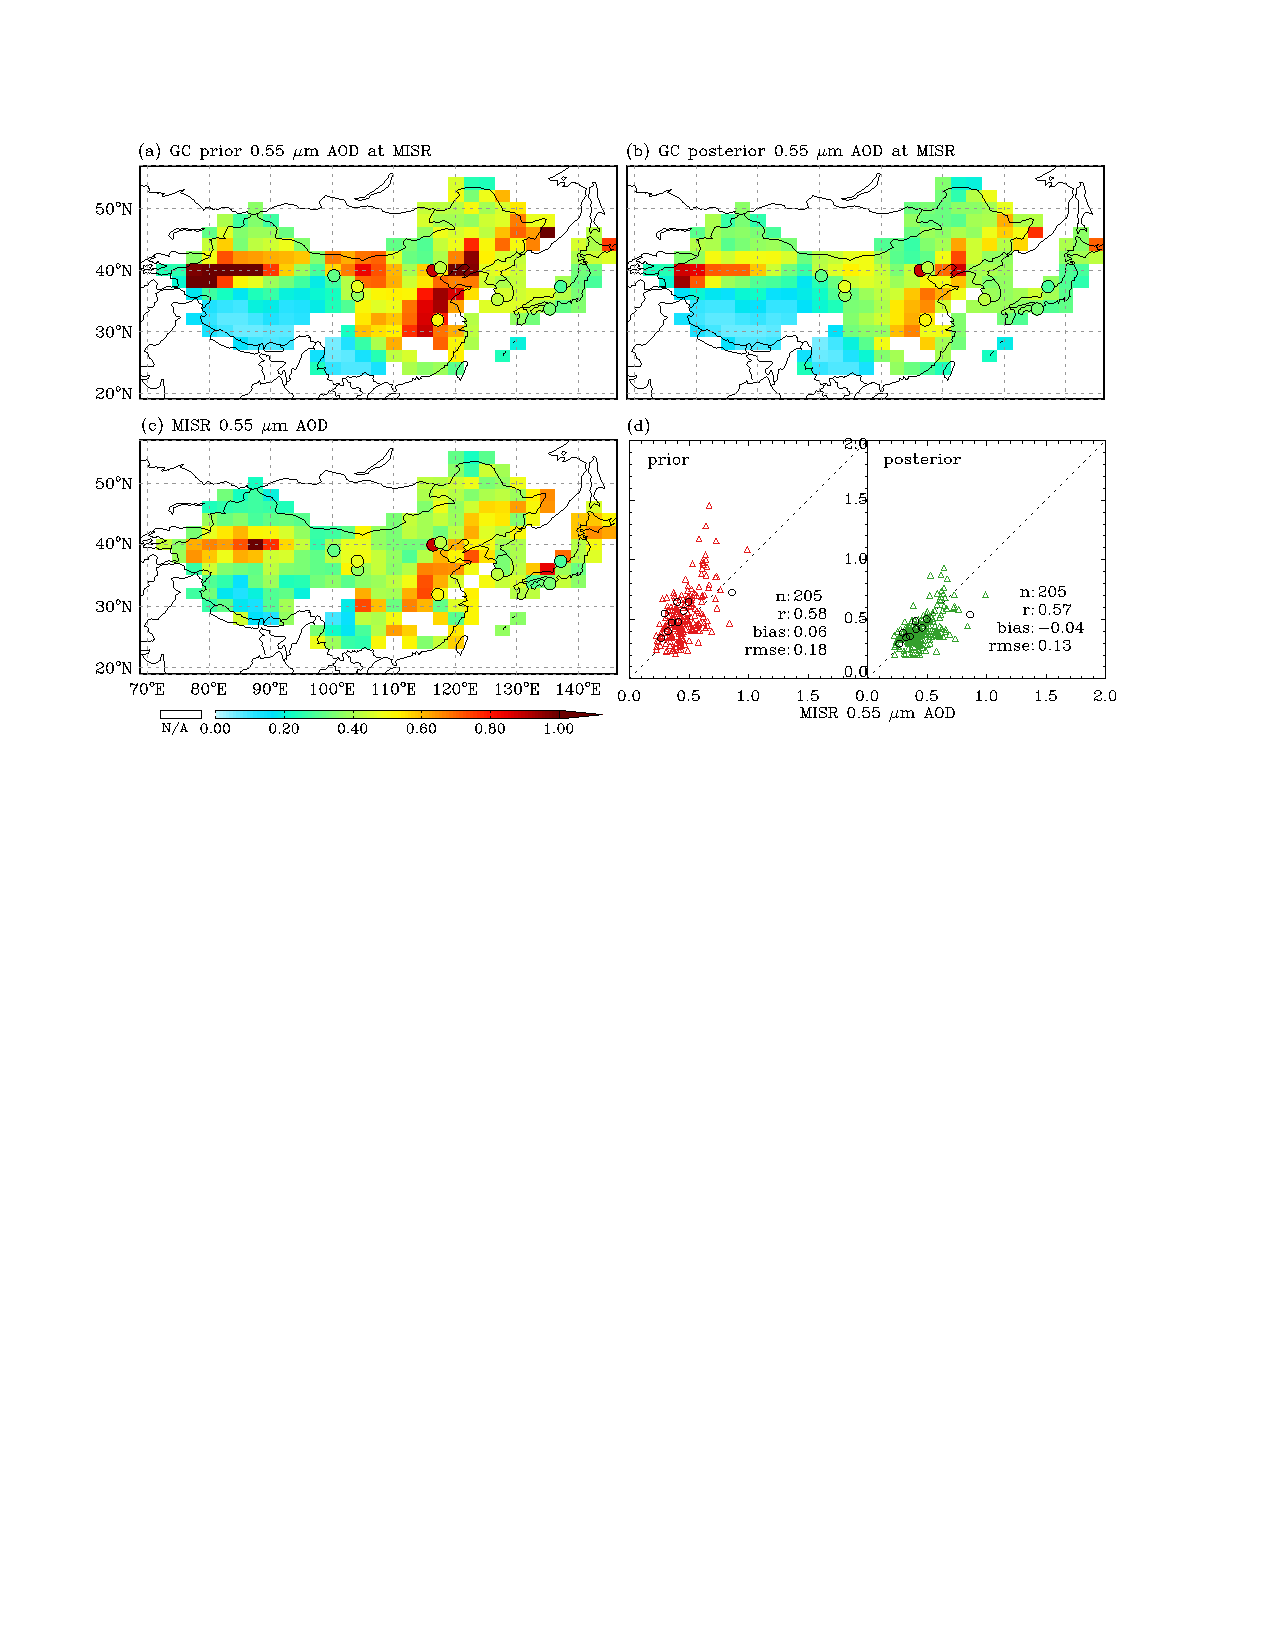
\includegraphics[width={0.9\textwidth}]{figures/a7.pdf}  
  \caption{Comparison of the prior and posterior GEOS-Chem simulation of 0.55 $\mu$m AOD with the level 3 MISR 0.55 $\mu$m AOD for the period April 2008. (a) The prior GEOS-Chem 0.55 $\mu$ AOD that are sampled coincidentally with MISR AODs for the period of April 2008. Also overlaid circles are the monthly AOD averages at 0.55 $\mu$m observed from the nine AEORNET sites shown in Figure \ref{fig:aeronet}. (b) Same as (a) but for the monthly average of posterior GEOS-Chem AOD. (c) Monthly average of the Level 3 daily MISR 0.55 $\mu$m AOD.  (d) Scatter plot the GEOS-Chem AOD versus the MISR AOD before (red scatters) and after optimization (green scatters), in which each point indicates an AOD pair over a model grid cell with value over 0.2. Also shown are the statistics including number of sampled pairs (n), correlation coefficient (R), bias and root-mean-square-error (rmse). Comparisons of the monthly GEOS-Chem AOD versus AERONET AOD are also included as the black circles; each circle indicates an AOD pair over an individual site.}
  \label{fig:misr1}
 \end{figure}

 The monthly averages of prior and posterior GEOS-Chem 0.55 $\mu$m AOD
 mapped in Figure \ref{fig:misr1}a-b are sampled coincidently to the MISR AOD.
 A comparison with the MISR AOD shows GEOS-Chem simulation with prior aerosol emissions
 overestimates AOD over both the desert and industrial regions.
 The posterior simulation is slightly more in agreement with MISR AOD.
 To facilitate the comparison of model with MISR AOD, we also include, as Figure \ref{fig:misr1}d,
 the scatterplots of the AOD for each GEOS-Chem grid cell with values larger than 0.2
 by considering the larger retrieval uncertainty in the low AOD conditions [Kahn et al., 2005].
 While the correlation coefficients remain about the same,
 both absolute bias and rmse are reduced about 30\%.

 \subsection{Comparisons with OMI Column \ce{SO2} and \ce{NO2}}

 The improvement in the optimized aerosol emissions is also exhibited
 in the comparison of simulated trace gases to the satellite retrievals from OMI.
 The GEOS-Chem \ce{SO2} simulations are assessed with OMI Level 3 daily products
 of planetary boundary layer (PBL) \ce{SO2} column gridded
 with 0.25$^{\circ}$ by 0.25$^{\circ}$ resolution.
 We average the OMI \ce{SO2} column retrievals into GEOS-Chem 2$^{\circ}$ by 2.5$^{\circ}$ grid cells
 and take the monthly average for comparison, which are shown in Figure \ref{fig:omso2}c.
 Figure \ref{fig:omso2}a and \ref{fig:omso2}b show model prior and posterior \ce{SO2} column
 that are coincidentally sampled with OMI retrievals.
 Figure \ref{fig:omso2}d illustrates the quantitative analysis for OMI \ce{SO2} retrievals
 larger than $1.0 \times 10^{16}$ molec cm$^{-2}$.
 With the optimized emission estimates, the bias and RMSE are reduced
 from 0.81 and 0.61 to – 0.28 and 0.38 ($10^{16}$molec cm$^{-2}$), respectively,
 along with an increase of correlation coefficient from 0.68 to 0.73. 

 %% Validation against OMI SO2
 \begin{figure}[t]
  \centering
  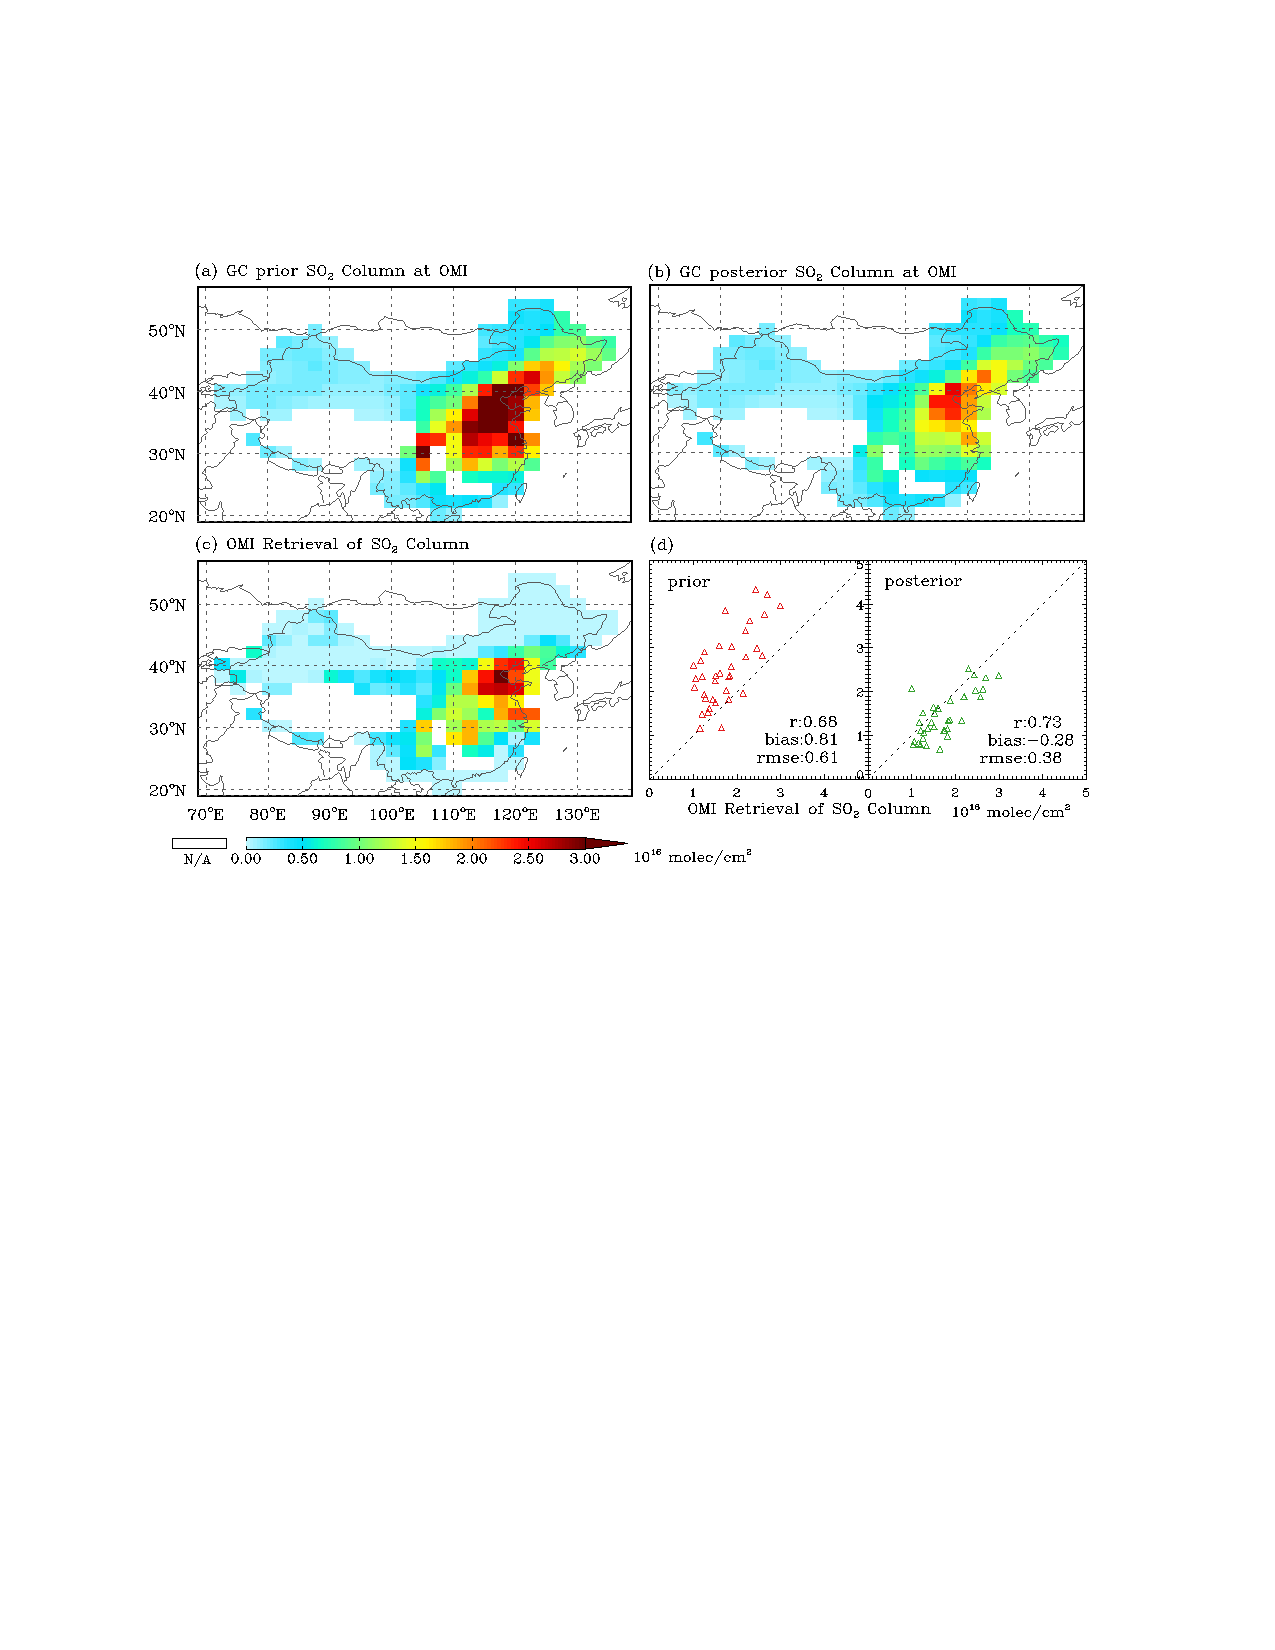
\includegraphics[width={0.9\textwidth}]{figures/a8.pdf}
  \caption{Same as figure \ref{fig:misr1} but for comparison of the GEOS-Chem \ce{SO2} simulation with OMI column \ce{SO2} retrievals for the period of April 2008. The OMI planetary boundary layer (PBL) column \ce{SO2} from the Level 3 daily products with 0.25$^{\circ}$ by 0.25$^{\circ}$ resolutions are aggregated into GEOS-Chem grid cells.}
  \label{fig:omso2}
 \end{figure}

 %% Validation against OMI NO2
 \begin{figure}[t]
  \centering
  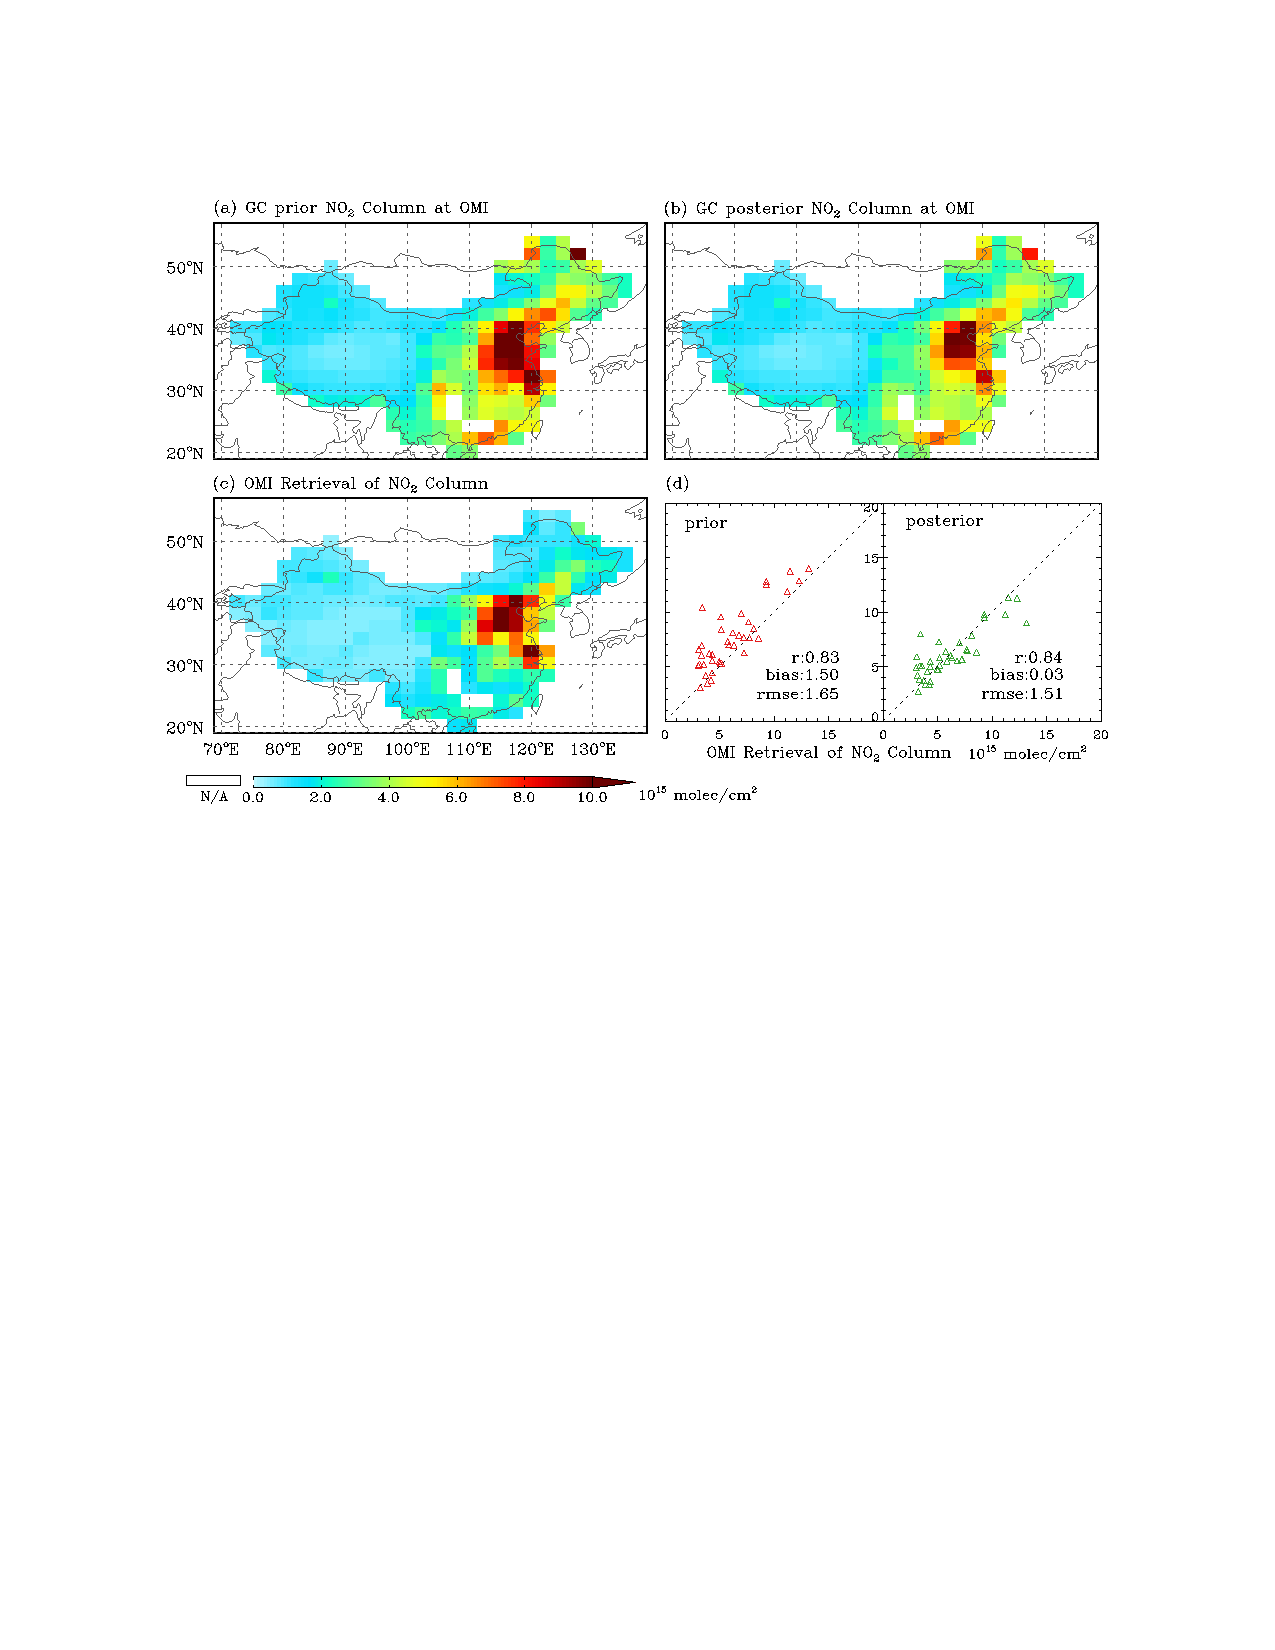
\includegraphics[width={0.9\textwidth}]{figures/a9.pdf}
  \caption{Same figure \ref{fig:misr1} but for comparison of the GEOS-Chem \ce{NO2} simulation with OMI column \ce{NO2} retrievals for the period of April 2008.  The OMI tropospheric column \ce{NO2} from Level 2 daily products with 0.25$^{\circ}$ by 0.25$^{\circ}$ resolutions are aggregated into GEOS-Chem grid cells.}
  \label{fig:omno2}
 \end{figure}

 We evaluate the model simulation of \ce{NO2} with OMI Level 2 products of
 \ce{NO2} tropospheric column over 0.25$^{\circ}$ by 0.25$^{\circ}$ grid cells.
 Recent studies suggested that the uncertainty in OMI \ce{NO2} tropospheric column retrievals
 is about 40\% with an about 15\% positive systematical bias
 [Boersma et al., 2008; Celarier et al., 2008].
 Following Lin et al. [2010], we apply a factor of 0.85 to OMI \ce{NO2} retrievals
 in our comparison to correct the bias.
 Figure \ref{fig:omno2} shows the comparison of GEOS-Chem \ce{NO2} columns
 with re-gridded OMI \ce{NO2} retrievals.
 Similarly, we also perform the quantitative analysis, as in Figure \ref{fig:omno2}d,
 for OMI \ce{NO2} column retrievals larger than $3.0 \times 10^{15}$ molec cm$^{-2}$.
 While the correlation coefficient remains about the same, the bias (RMSE) is reduced
 from 1.50 (1.65) to 0.03 (1.51) (units: $10^{15}$ molec cm$^{-2}$) after constraining aerosol emissions. 

 \subsection{Comparisons with near-surface aerosol mass concentrations}

 The accuracy of the sulfate-nitrate-ammonium (SNA) aerosol simulation
 is in part determined by the representation of the emissions of \ce{SO2} and \ce{NOx} and \ce{NH3},
 and hence GEOS-Chem simulations with constrained emissions should
 provide overall an improved simulation of SNA.
 Figure \ref{fig:sna} shows the comparison of daily near-surface SNA mass concentration
 from the prior and posterior GEOS-Chem simulations with measurements
 over Qingdao (120.34$^{\circ}$ E, 36.06$^{\circ}$ N), China.
 The error bars for the GEOS-Chem curves indicate the diurnal standard deviation.
 An overestimation in the prior model surface SNA simulations is found
 when comparing with observed counterparts, which shows a bias of 14.28 $\mu$g m$^{-3}$,
 RMSE of 21.84 $\mu$g m$^{-3}$, and correlation coefficient of 0.46.
 Such bias is significantly reduced to 0.34 $\mu$g m$^{-3}$
 in the simulation with top-down constrained emissions,
 along with a 50\% decrease in RMSE and a 28\% increase in correlation coefficient.

 %% Validation against surface SNA
 \begin{figure}[ht]
  \centering
  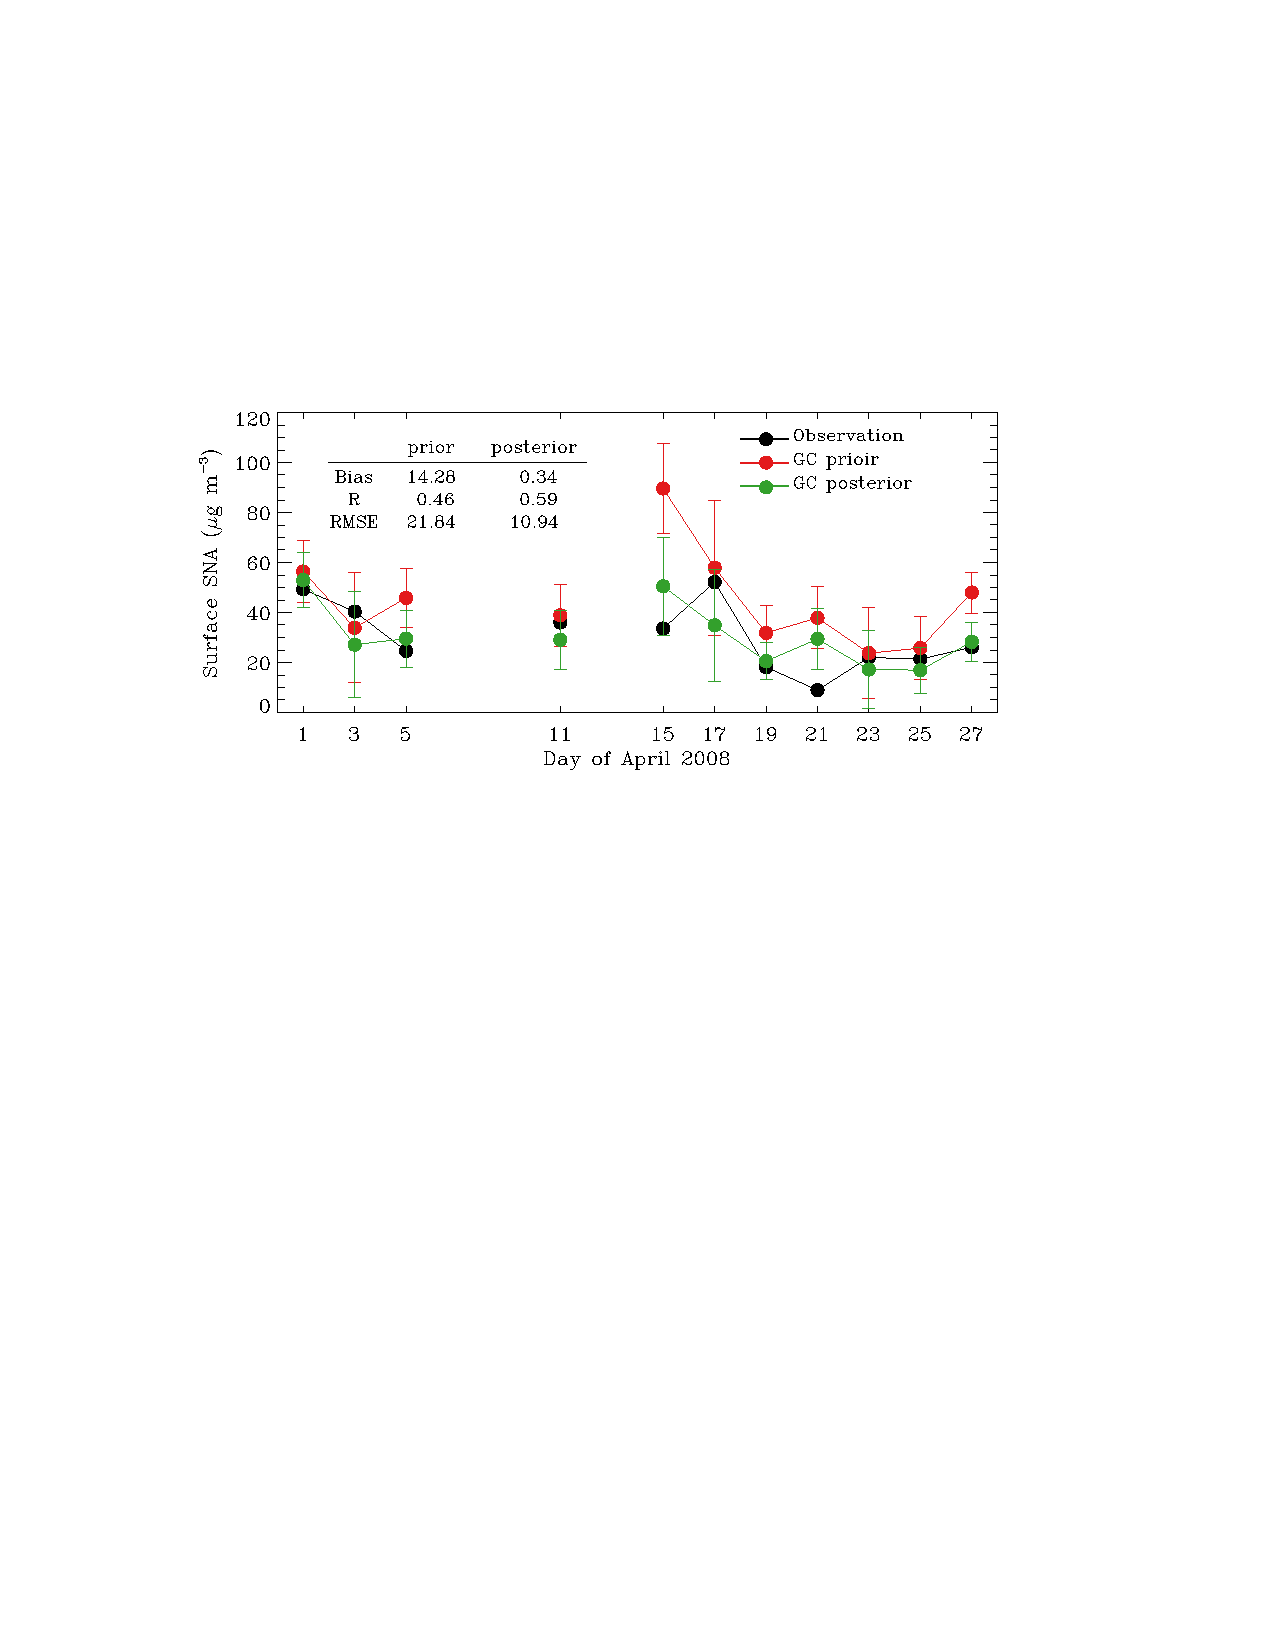
\includegraphics[width={0.8\textwidth}]{figures/a10.pdf}
  \caption{Comparison of the GEOS-Chem surface mass concentration of sulfate-nitrate-ammonium (SNA) aerosols with ground-based observations over Qingdao (120.34$^{\circ}$ E, 36.06$^{\circ}$ N), China. Discontinuity in time series is due to missing or quality filtered observations.}
  \label{fig:sna}
 \end{figure}

 %% Validation against surface PM10
 \begin{figure}[t]
  \centering
  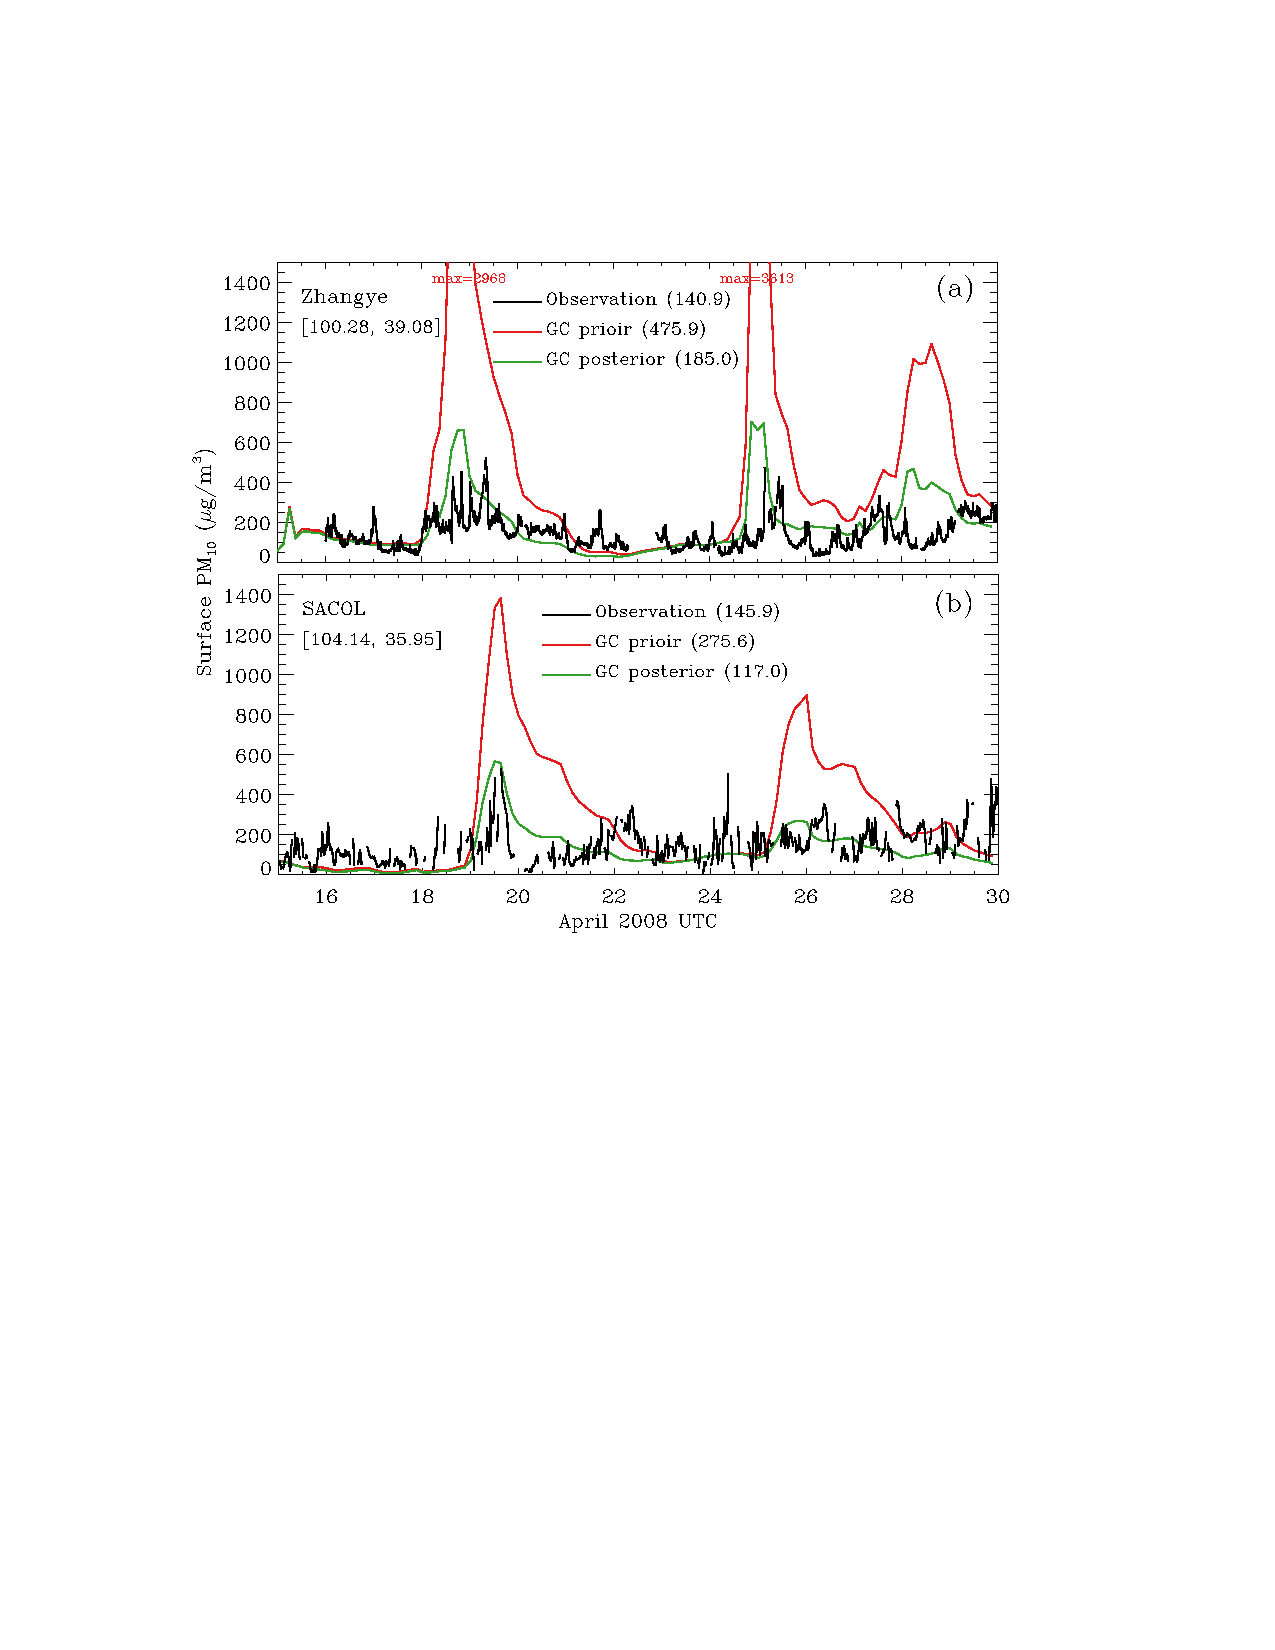
\includegraphics[width={0.95\textwidth}]{figures/a11.pdf}
  \caption{Time serial plot of the GEOS-Chem simulated surface PM\textsubscript{10} concentrations by prior (red) and posterior (red) aerosol emissions compared with the \textit{in situ} measured PM\textsubscript{10} (black) over Zhangye (a) and SACOL (b) stations for 15 – 30 April 2008; also shown are the average values over same the period. Discontinuity in time series is due to missing or quality filtered observations.}
  \label{fig:pm10}
 \end{figure}

 The mass concentration over or near the dust source regions
 where the anthropogenic emissions are small is most sensitive to the dust mass loading,
 and thus can be an indicator of the dust emissions in the first order.
 Figure \ref{fig:pm10} shows the prior and posterior GEOS-Chem surface
 PM\textsubscript{10} mass concentration compared with the ground-based measurements
 from the 2008 China-U.S. joint field experiment [Ge et al., 2010] over two the AERONET sites
 in Figure \ref{fig:aeronet}a-b, i.e., Zhangye (100.28$^{\circ}$ E, 39.08$^{\circ}$ N)
 and SACOL (204.14$^{\circ}$ E, 35.95$^{\circ}$ N), which are located
 on the downwind boundaries of the Gobi deserts.
 Based on the availability of the measurements data, comparisons are for the period of 15 $-$ 30 April 2008.
 The measured surface PM\textsubscript{10} shows a strong daily variation.
 A strong dust event during 18$-$20 April can be found over both stations with
 PM\textsubscript{10} exceeding 400 $\mu$g m$^{-3}$.
 Two additional dust events with PM\textsubscript{10} over 400 $\mu$g m$^{-3}$ occurred during
 24$-$26 and 29$-$30 April.
 The prior simulation generally captures the daily variation pattern
 but significantly overestimates the surface PM\textsubscript{10} for those dust events;
 prior simulated PM\textsubscript{10} reaches up to around 3000 $\mu$g m$^{-3}$ over Zhangye
 and 1000 $\mu$g m$^{-3}$ over SACOL for the dust events during 18$-$20 and 24$-$26 April 2008.
 The two-week averages show the prior simulation overestimates PM\textsubscript{10}
 a factor of 2 over Zhangye and a factor of 1 over SACOL in the magnitude.
 After optimization, the relative biases in the PM\textsubscript{10} simulation are reduced to about 25\%.
 Moreover, the comparison of the time series of the PM\textsubscript{10} also shows that
 the model value with top-down emissions has much better agreement
 with the measurements in terms of temporal variation.

 \subsection{Evaluation summary}

 A summary of evaluations of the prior and posterior model simulations
 is illustrated in Figure \ref{fig:taylor} using a Taylor diagram [Taylor, 2001].
 Taylor diagram provides a statistical summary of the model performance
 in terms of correlation coefficients (R), centralized root-mean-square difference (RMSD),
 and ratio of standard deviations between model and observations (or normalized standard deviation, NSD).
 The latter two quantities reflect how well model captures
 the temporal or/and spatial variation of observations.
 In the Taylor diagram, cosine of polar angles represents R, and radius (dotted-contour) indicates NSD.
 Thus, the reference point (black circle) where R and NSD are unity represents observations,
 and the distance (dashed-contour) of certain point from which indicates the RMSD.
 Considering that the Taylor diagram itself is not able to show the statistical bias,
 we use different colors for each data points to indicate their respective relative biases.
 The data points labeled from 1 to 6 indicate comparisons between model and observations of
 (1) AERONET AOD at 0.55 $\mu$m,
 (2) MISR 0.55 $\mu$m AOD,
 (3) OMI retrievals of \ce{SO2} Column,
 (4) OMI retrievals of \ce{NO2} Column,
 (5) surface concentration of SNA over Qingdao, and
 (6) surface concentration of PM\textsubscript{10} over Zhangye and SACOL, respectively.
 Square and circles represent the evaluations for prior and posterior GEOS-Chem simulations, respectively.

 %% Validation Taylor diagram
 \begin{figure}[t]
  \centering
  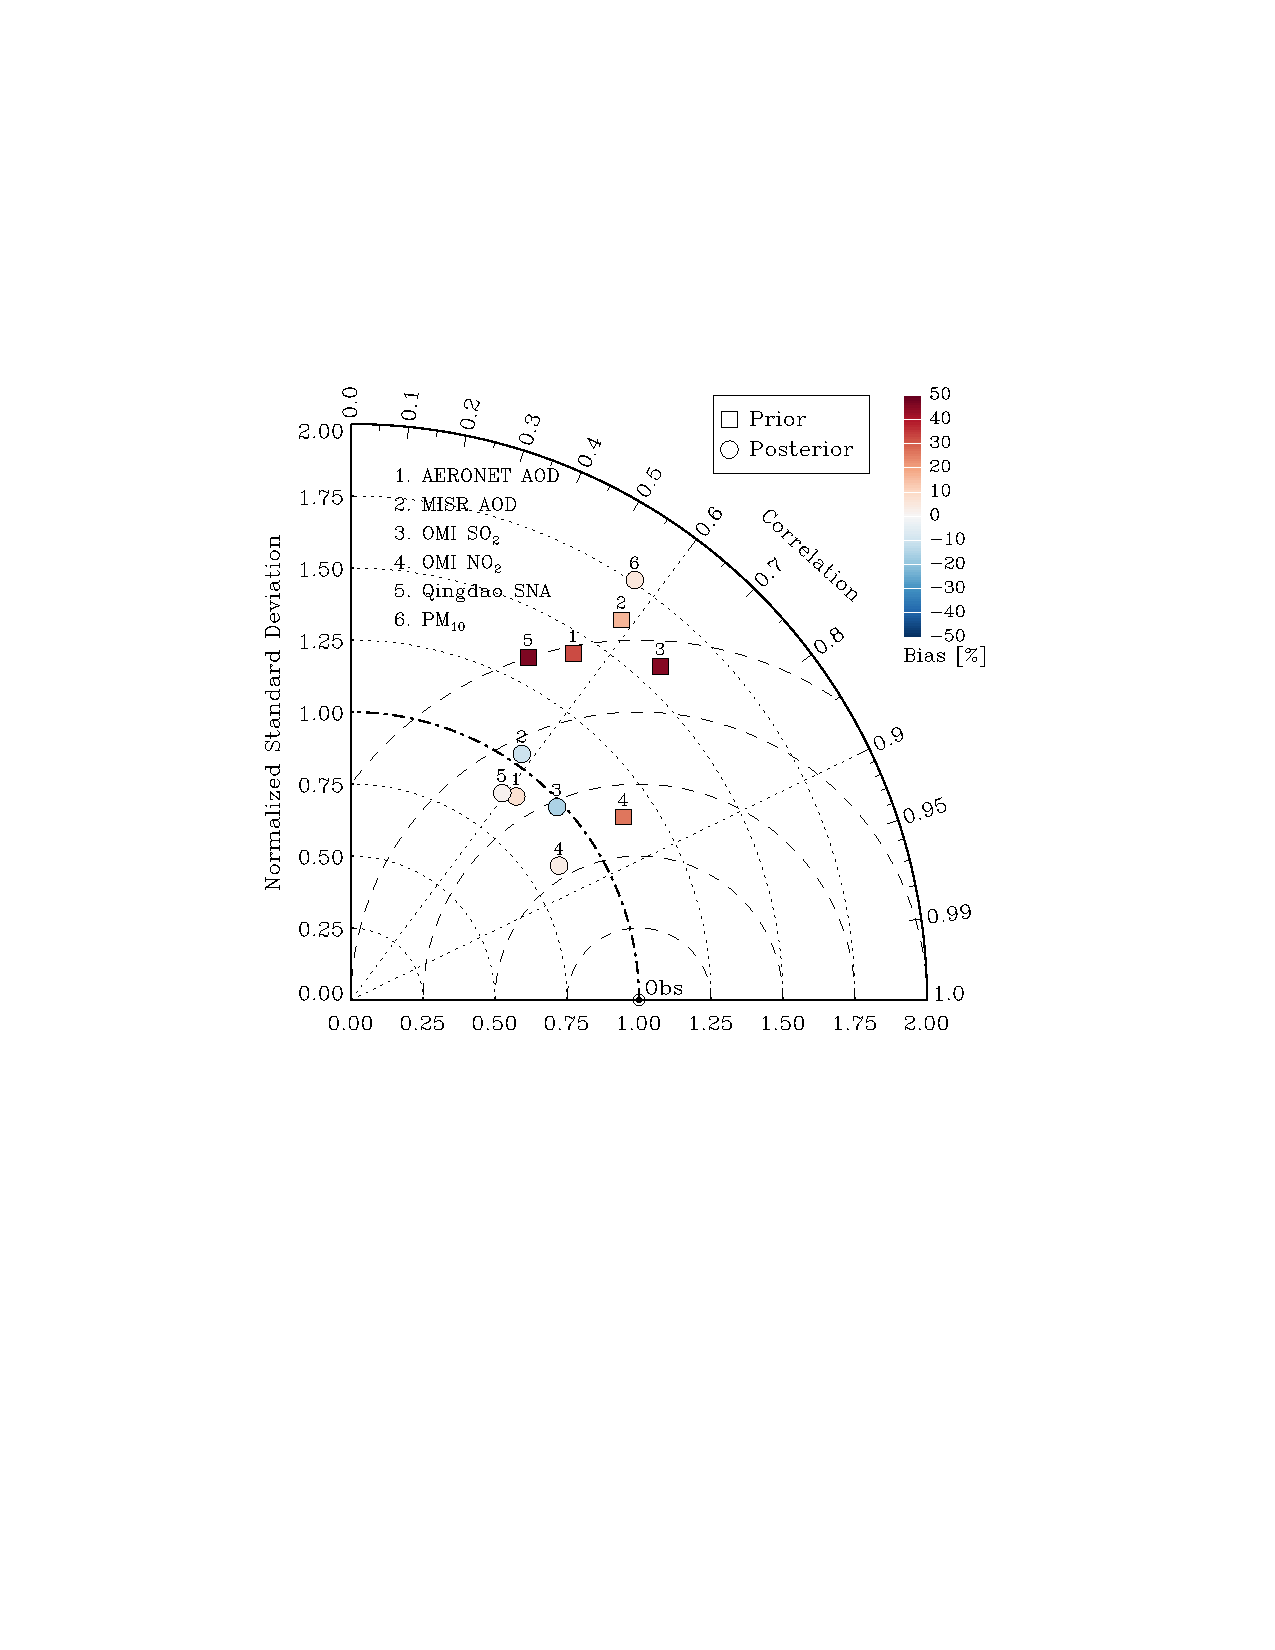
\includegraphics[width={0.66\textwidth}]{figures/a12.pdf}
  \caption{Taylor diagram for the model evaluations before (squares) and after (circles) optimization when comparing against (1) AERONET AOD at 0.55 $\mu$m, (2) MISR 0.55 $\mu$m AOD, (3) OMI column \ce{SO2}, (4) OMI column \ce{NO2}, (5) surface SNA concentrations at Qingdao site, and (6) surface PM\textsubscript{10} concentrations measured at Zhangye and SACOL sites. The color coded on each point indicates the relative bias. It should be noted that the ratio of standard deviations and correlation coefficient between prior GEOS-Chem simulated and measured surface PM\textsubscript{10} over Zhangye and SACOL are 6.5 and 0.45, which makes the point number 6 for the prior simulation far beyond the range of this Taylor diagram. }
  \label{fig:taylor}
 \end{figure}

 It should be noted that the NSD between prior GEOS-Chem simulated
 and measured surface PM\textsubscript{10} during the China-U.S. joint field campaign
 is about 6.5 (and R of 0.45) that are significantly beyond the range of this Taylor diagram.
 Consequently, the square point of number 6 is not shown in the diagram.
 It is clear from the Taylor diagram that the circular points (posterior simulation)
 are generally closer than the square points (prior simulation) to the reference point
 and to the unity curve of NSD, and have remarkably decreased bias.
 Evaluations with all those independent observations indicate a notable
 improvement in the model simulation, reflecting a better estimate of aerosol emissions.

\section{Implications of Results}

  Interpretation of our inversion results can be from two different perspectives. 
First, if assuming that bottom-up anthropogenic emissions are the best estimates for their base years (mostly 2006), 
the reduction in the top-down emissions over China for April 2008 may indicate a decrease of emissions for April from 2006 to 2008. 
This conjecture is supported by the finding of significant decrease of AOD from 2006 to 2008 over the eastern China, 
shown both in the MODIS and MISR Level 3 gridded products (Figure \ref{fig:aodchange}),
if we assume that the impact on AOD of meteorological differences between the two years is smaller than the differences in emissions.
Furthermore, a slight increase of AOD over the Southeastern China (Figure \ref{fig:aodchange}) 
is also found to be consistent to the increase in the top-down emission estimates (Figure \ref{fig:ems1}). 
In contrast to the first interpretation, the second one is that the difference of actual emissions between 2008 and their base year (2006)
are smaller than the magnitude of adjustments in the optimization, 
and hence our results imply that the priori bottom-up emissions might be artificially overestimated. 
We further elucidate those two points below with a literature survey (data are summarized in Table 4).

 %% Satellite AOD changes
 \begin{figure}[t]
  \centering
  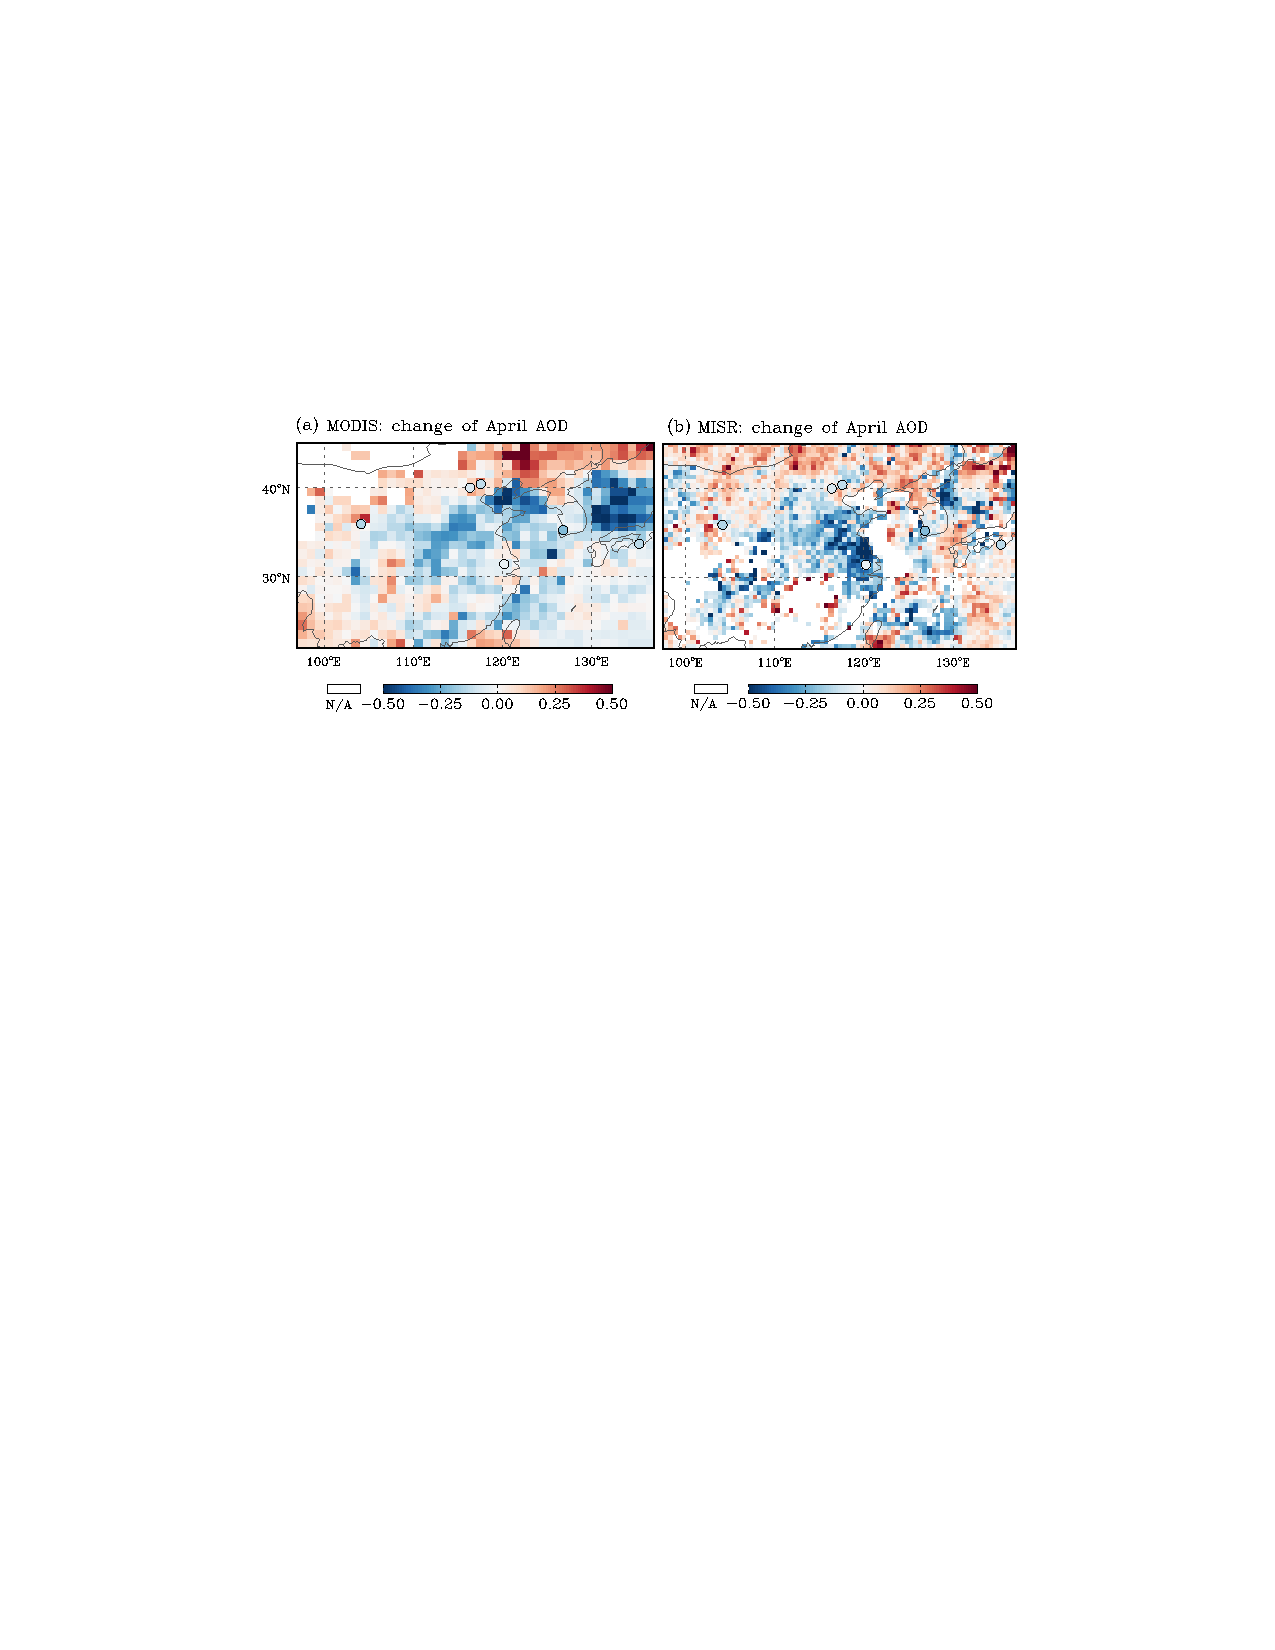
\includegraphics[width={0.90\textwidth}]{figures/a13.pdf}
  \caption{Change of April monthly 0.55 $\mu$m AOD from 2006 to 2008 from MODIS (a) and MISR (b) Level 3 daily products.}
  \label{fig:aodchange}
 \end{figure}

 \subsection{\ce{SO2}}

  The INTEX-B inventory by Zhang et al. [2009] reported an annual production of 31.02 Tg from anthropogenic sources over China. 
A decrease trend of China SO2 emissions from 2006 to 2008 has been found based on bottom-up estimates by Lu et al. [2010] from 33.2 to 31.3 ( \~5.8\% decrease) Tg yr$^{-1}$
and by China Ministry of Environmental Protection [2009] (hereafter referred to MEP-2008) from 25.9 to 23.2 Tg yr$^{-1}$ (\~10.4\% decrease).
With OMI \ce{SO2} retrievals, Lu et al. [2010] found the dramatic reduction of \ce{SO2} emissions over the northern China for the same period. 
Similar to this study, Lu et al. [2010] also presented that the reductions is more significant over the Eastern China. 
They attribute some reduction to the widespread installation of flue-gas desulfurization devices in power plants, which is enforced by the China government since 2006. 
Evidences for the reduction trend of \ce{SO2} emission also include the reduction of \ce{SO2} column from 2006 observed by both SCIAMACHY and OMI satellite sensors [Lu et al., 2011].
With the same SCIAMACHY and OMI \ce{SO2} retrievals, Lee et al. [2011] obtained top-down estimates of China SO2 emissions, 
which are lower by 50\% for SCIAMACHY and 30\% for OMI than the INTEX-B inventory. 
Thus, the reduction of 33.5\% in the top-down China \ce{SO2} emissions of this work can be interpreted by the joint contribution of a decrease trend and a possible overestimation in INTEX-B bottom-up inventory.

 \subsection{\ce{NH3} } 
  The \ce{NH3} emissions over China have not changed much since 2000, as confirmed by the REAS inventory [Ohara et al., 2007]. 
Our study shows an overall decrease of 34.5\% in the optimized from the TRACE-P 2000 inventory [Streets et al., 2003], 
which may indicate an overestimation in the TRACE-P inventory. 
As shown in Table 4, the total amount of the constrained \ce{NH3} emission (0.72 Tg Mon$^{-1}$) for April 2008 is quite close to a recent bottom-up estimates (0.71 Tg Mon$^{-1}$) by Huang et al., [2012]. 
Huang et al., [2012] also pointed out that the TRACE-P 2000 inventory significantly overestimates the \ce{NH3} emission by applying an overestimated emission factor across the whole country. 

 \subsection{\ce{NOx}} 
  Lin et al. [2010] constrained Chinese anthropogenic emissions of \ce{NOx} July 2008 with tropospheric \ce{NO2} retrievals from GOME-2 and OMI instruments.
They found the top-down emissions are (10$-$15\%) lower than the \textit{a priori} near Beijing (in agreement with results from Mijling et al. [2009]),
in the northeastern provinces and along the east coast; yet they exceed the a priori over many inland regions. 
Overall, they presented a best top-down estimate of annual \ce{NOx} production is 6.8 Tg N, or 22.34 Tg NO2, which is slightly higher than the \textit{a priori}. 
While the change in \ce{NOx} emission over China remains controversy, the 18.8\% difference of posterior NOx emissions from the bottom-up still lies in the 31\% uncertainty of the inventory [Zhang et al., 2009].
We argue bottom-up \ce{NOx} estimate from INTEX-B inventory could have a possible overestimation.   

 \subsection{BC and OC}  
  Major emitting sectors of BC and OC are coal and biofuel combustion by industry, residential, and transportation activities. 
The trend of BC and OC emissions in China during recent years are controlled by the balance between decrease in emission factor which is pertain to improved technology and increase in coal and fuel consumptions. 
According to MEP-2008 [Environmental Protection Administration, 2009], the annual smoke emission in China decreased by about 17.2\% from 2006 to 2008. 
While BC and OC emissions estimated by Lu et al. [2011] and Zhao et al. [2013] remain almost same between 2006 and 2008, Qin and Xie [2012] reported a 3.8\% increase. 
The top-down BC emission is 0.10 Tg mon$^{-1}$ (or 1.509 Tg yr$^{-1}$ based on the monthly variation in INTEX-B inventory), which is smaller than that in INTEX-B, but close to estimates of 1.61 Tg yr$^{-1}$ by Qin and Xie [2012] and 1.68 Tg yr$^{-1}$ by Lu et al. [2011]. 
In terms of China OC emission estimates for 2008, Lu et al. [2011] suggested a slightly larger value (3.37 Tg yr$^{-1}$) while Zhao et al. [2013] indicated a smaller value (2.8 Tg yr$^{-1}$) than INTEX-B (3.22 Tg yr$^{-1}$).  Our OC emission estimate (0.18 Tg mon$^{-1}$ or 2.92 Tg yr$^{-1}$) is within their reported range. 
It is noted that the uncertainty for OC emissions is reported to be very large: 258\% in INTEX-B [Zhang et al., 2009], $-$43\% to 80\% by Lu et al. [2011], and $-$42\% to 114\% in a recent study by Zhao et al. [2013].

 \subsection{Mineral dust} 
  The \~50\% reduction in the posterior dust emission estimates suggests the use of DEAD mobilization scheme with GOCART source function possibly tends to produce a systematic positive bias over the Taklimakan and Gobi deserts regions over the northwestern China, 
even it works reasonably for the United States \citep{fairlie07}. 
Similar results have been also found in top-down dust emission estimates by MODIS aerosol retrievals [Wang et al., 2012], 
and constrained dust emissions by surface PM measurements [Ku and Park, 2011]. 
Such overestimation by the dust mobilization scheme is also reflected through comparison GEOS-Chem AOD 
(as in Figure \ref{fig:aeronet}) and surface PM10 concentration (as in Figure \ref{fig:pm10}) with in situ measurements near the dust source regions. 


\section{Summary}

 This study presents a two-stage inversion scheme to explore the capacity of using satellite radiance for inversion of species-specific aerosol emissions.
 Firstly, we prepare the observational constraints of AOD using an advanced aerosol retrieval algorithm,
 which integrates the GEOS-Chem aerosol optical properties to the MODIS observed radiance [Wang et al., 2010].
 Secondly, the adjoint of the GEOS-Chem chemical transport model is applied to statistically optimize aerosol emission estimates using these AOD retrievals.
 Thus, the MODIS radiances are essentially used to optimize the estimates of the emitted aerosol tracers and precursors.
 We illustrate our concept first with an idealized numerical experiment,
 and subsequently demonstrate the feasibility and practicability of the proposed scheme by applying it to optimize aerosol emission inventories over China during April 2008.
 Emissions of \ce{SO2}, \ce{NH3}, \ce{NOx}, BC and OC from anthropogenic sources,
 which significantly influence the aerosol simulation, are selected to be constrained at a spatial resolution of 2$^{\circ}$ by 2.5$^{\circ}$ and a monthly temporal resolution.
 Mineral dust production from combined natural and disturbed sources are optimized at the same spatial resolution but with a daily temporal resolution.
 Independent observations from both satellite remote sensing and ground-based observations are used to assess the inversion results through their comparisons with relevant GEOS-Chem simulations using prior and posterior emission estimates. 

The inversion yields posterior best estimates of 1.73 Tg for \ce{SO2}, 0.72 Tg for \ce{NH3}, 1.38 Tg for NOx, 0.10 Tg for BC, and 0.18 for OC from anthropogenic sources, and 8.3 Tg for combined natural and disturbed mineral dust.
 These show notable decreases from their counterparts in the bottom-up inventories in amount (or percentage decrease): 0.87 Tg (33.5\%) for \ce{SO2}, 0.38 Tg (34.5\%) for \ce{NH3}, 0.32 Tg (18.8\%) for \ce{NOx}, 0.01 Tg (9.1\%) for BC, and 0.03 Tg (15.0\%) for OC.
 The total amount of the mineral dust emission is reduced by 56.4\% from 19.02 Tg simulated by the DEAD mobilization module.
 The distribution of emission scaling factors exhibits strong spatial variation for those anthropogenic-emitted tracers and considerable temporal variation for mineral dust.
 The use of top-down constrained emissions remarkably reduces the discrepancy between GEOS-Chem simulation and observational AOD constraints, in both spatial and temporal variation features.

 Resulting posterior estimates of emissions are evaluated with independent AOD observations from surface sites (AERONET) and satellite (MISR),
 \ce{SO2} and \ce{NO2} column retrievals from satellite (OMI), and surface SNA and PM\textsubscript{10} concentrations from ground-based measurements.
 While the prior simulation over China generally shows overestimation, the use of posterior emissions significantly enhances the consistency between simulations and those independent observations.
 The statistical analysis of those comprehensive comparisons summarized in the Taylor diagram shows an overall reduced bias and root-mean-squre difference along with increased correlation coefficient, further confirming the improvements in the posterior simulation and the effectiveness of the presented top-down scheme. 

 We attribute the differences between prior and posterior aerosol emissions to the change of emitted amount from the base year of those bottom-up inventories to the study period and/or the under/over-estimations in those inventories.
 Through comparisons with emissions over China reported by recent studies, we find that our inversion results are consistent with following finding:
 \begin{itemize}
 \item Anthropogenic \ce{SO2} emissions over China has been decreased by 5$-$10\% from 2006 to 2008;
 \item Anthropogenic BC/OC emissions may be slightly reduced;
 \item Anthropogenic emissions of \ce{SO2} and \ce{NOx} reported in the INTEX-B and \ce{NH3} from TRACE-P inventories could have been artificially overestimated;
 \item The DEAD mobilization scheme combined with GOCART dust source function, even works well over the United State \citep{farelie07}, seems to simulate mineral dust surface fluxes with a systematic positive bias.  
 \end{itemize}
  
 As a first attempt to invert species-specific emissions with satellite radiance, this study has a number of limitations.
 Those limitations may impact the uncertainty in posterior emissions, which is supposed to be smaller than uncertainty characterizing either a priori or observational constraints [Rodgers, 2000].
  While quantification of these is beyond the demonstrative purposes of this paper, we present a qualitative discussion as follows.
 First, in the stage of aerosol retrieval, we presume aerosol composition is unbiased, and contains errors only in the total amount.
 As the model inevitably has bias associating aerosol types, improvement of this assumption over regional to global scale can be obtained from innovative satellite measurements.
 Indeed, the radiance observations have potential information on the aerosol composition.
 For example, the spectral behavior of the radiance is used to discriminate smoke from mineral dust particles [King et al., 1999; Kaufman et al., 2002].
 Radiances measured from multi-viewing-angle are sensitive to aerosol particle size and nonsphericity [Kahn et al., 2005].
 Temporal variation and geographical location can also yield information about aerosol composition.
 For example, increase of AOD in semi-arid region may reflect the increase of dust, while change of AOD in the Eastern Asia may reflect the increase of industrial emission.
 Hence, as showed in this study, a combined use of the model-based knowledge of the dominant aerosol sources and the source-receptor relationship together with the satellite-based temporal variation of AOD at different locations can be a strong constraint for species-specific source estimates.
 Second, this study also assumes the sole cause of the radiance difference (or the AOD difference) is due to the uncertainty in aerosol emissions.
 However, other processes can contribute to the difference, e.g. aerosol transport, wet/dry deposition, diurnal variation, prescribed aerosol physical and optical properties, and errors in the meteorological fields and radiative transfer calculation, etc.
 The third assumption is related to the error covariance matrices that are specified as diagonal with errors based upon literature (but that themselves may have uncertainty).
 To properly address these issues in future, a logical next step would be to assimilate multiple-spectral and/or multi-angle satellite radiance to the CTM.
 Furthermore, errors in the processes including emission, transport, and deposition and radiative transfer, should be reasonably characterized and included in the optimization. 

The top-down inversion scheme using GEOS-Chem adjoint inverse modeling is a powerful tool to include observational constraints from different platforms for timely updating aerosol emissions.
 There is also a need of using combined tracer gas and aerosol measurements to simultaneously constrain the aerosol emissions and gas precursors.
 Encouraging results presented in this study reveal the potential of using aerosol observations from MODIS and MISR, \ce{SO2} and \ce{NO2} from OMI and other sensor, such as SCIAMACHY, in the inversion. Inclusion of those observations will undoubtedly add more information to the optimization of emission. 

